\chapter{System Design}
\section{Introduction}
The Student Portal system is designed to provide a unified platform for academic collaboration, resource sharing, and event management. This chapter details the architectural decisions, data models, and system workflows that form the foundation of the application.

Key design principles include:
\begin{itemize}
    \item Modular architecture for scalability
    \item Role-based access control for security
    \item Real-time communication capabilities
    \item AI-powered recommendation systems
    \item Cross-platform compatibility (web and mobile)
\end{itemize}

\section{Sequence Diagrams}
The following sequence diagrams illustrate key workflows in the Student Portal system:

\subsection{User Registration Process}
\begin{figure}[H]
    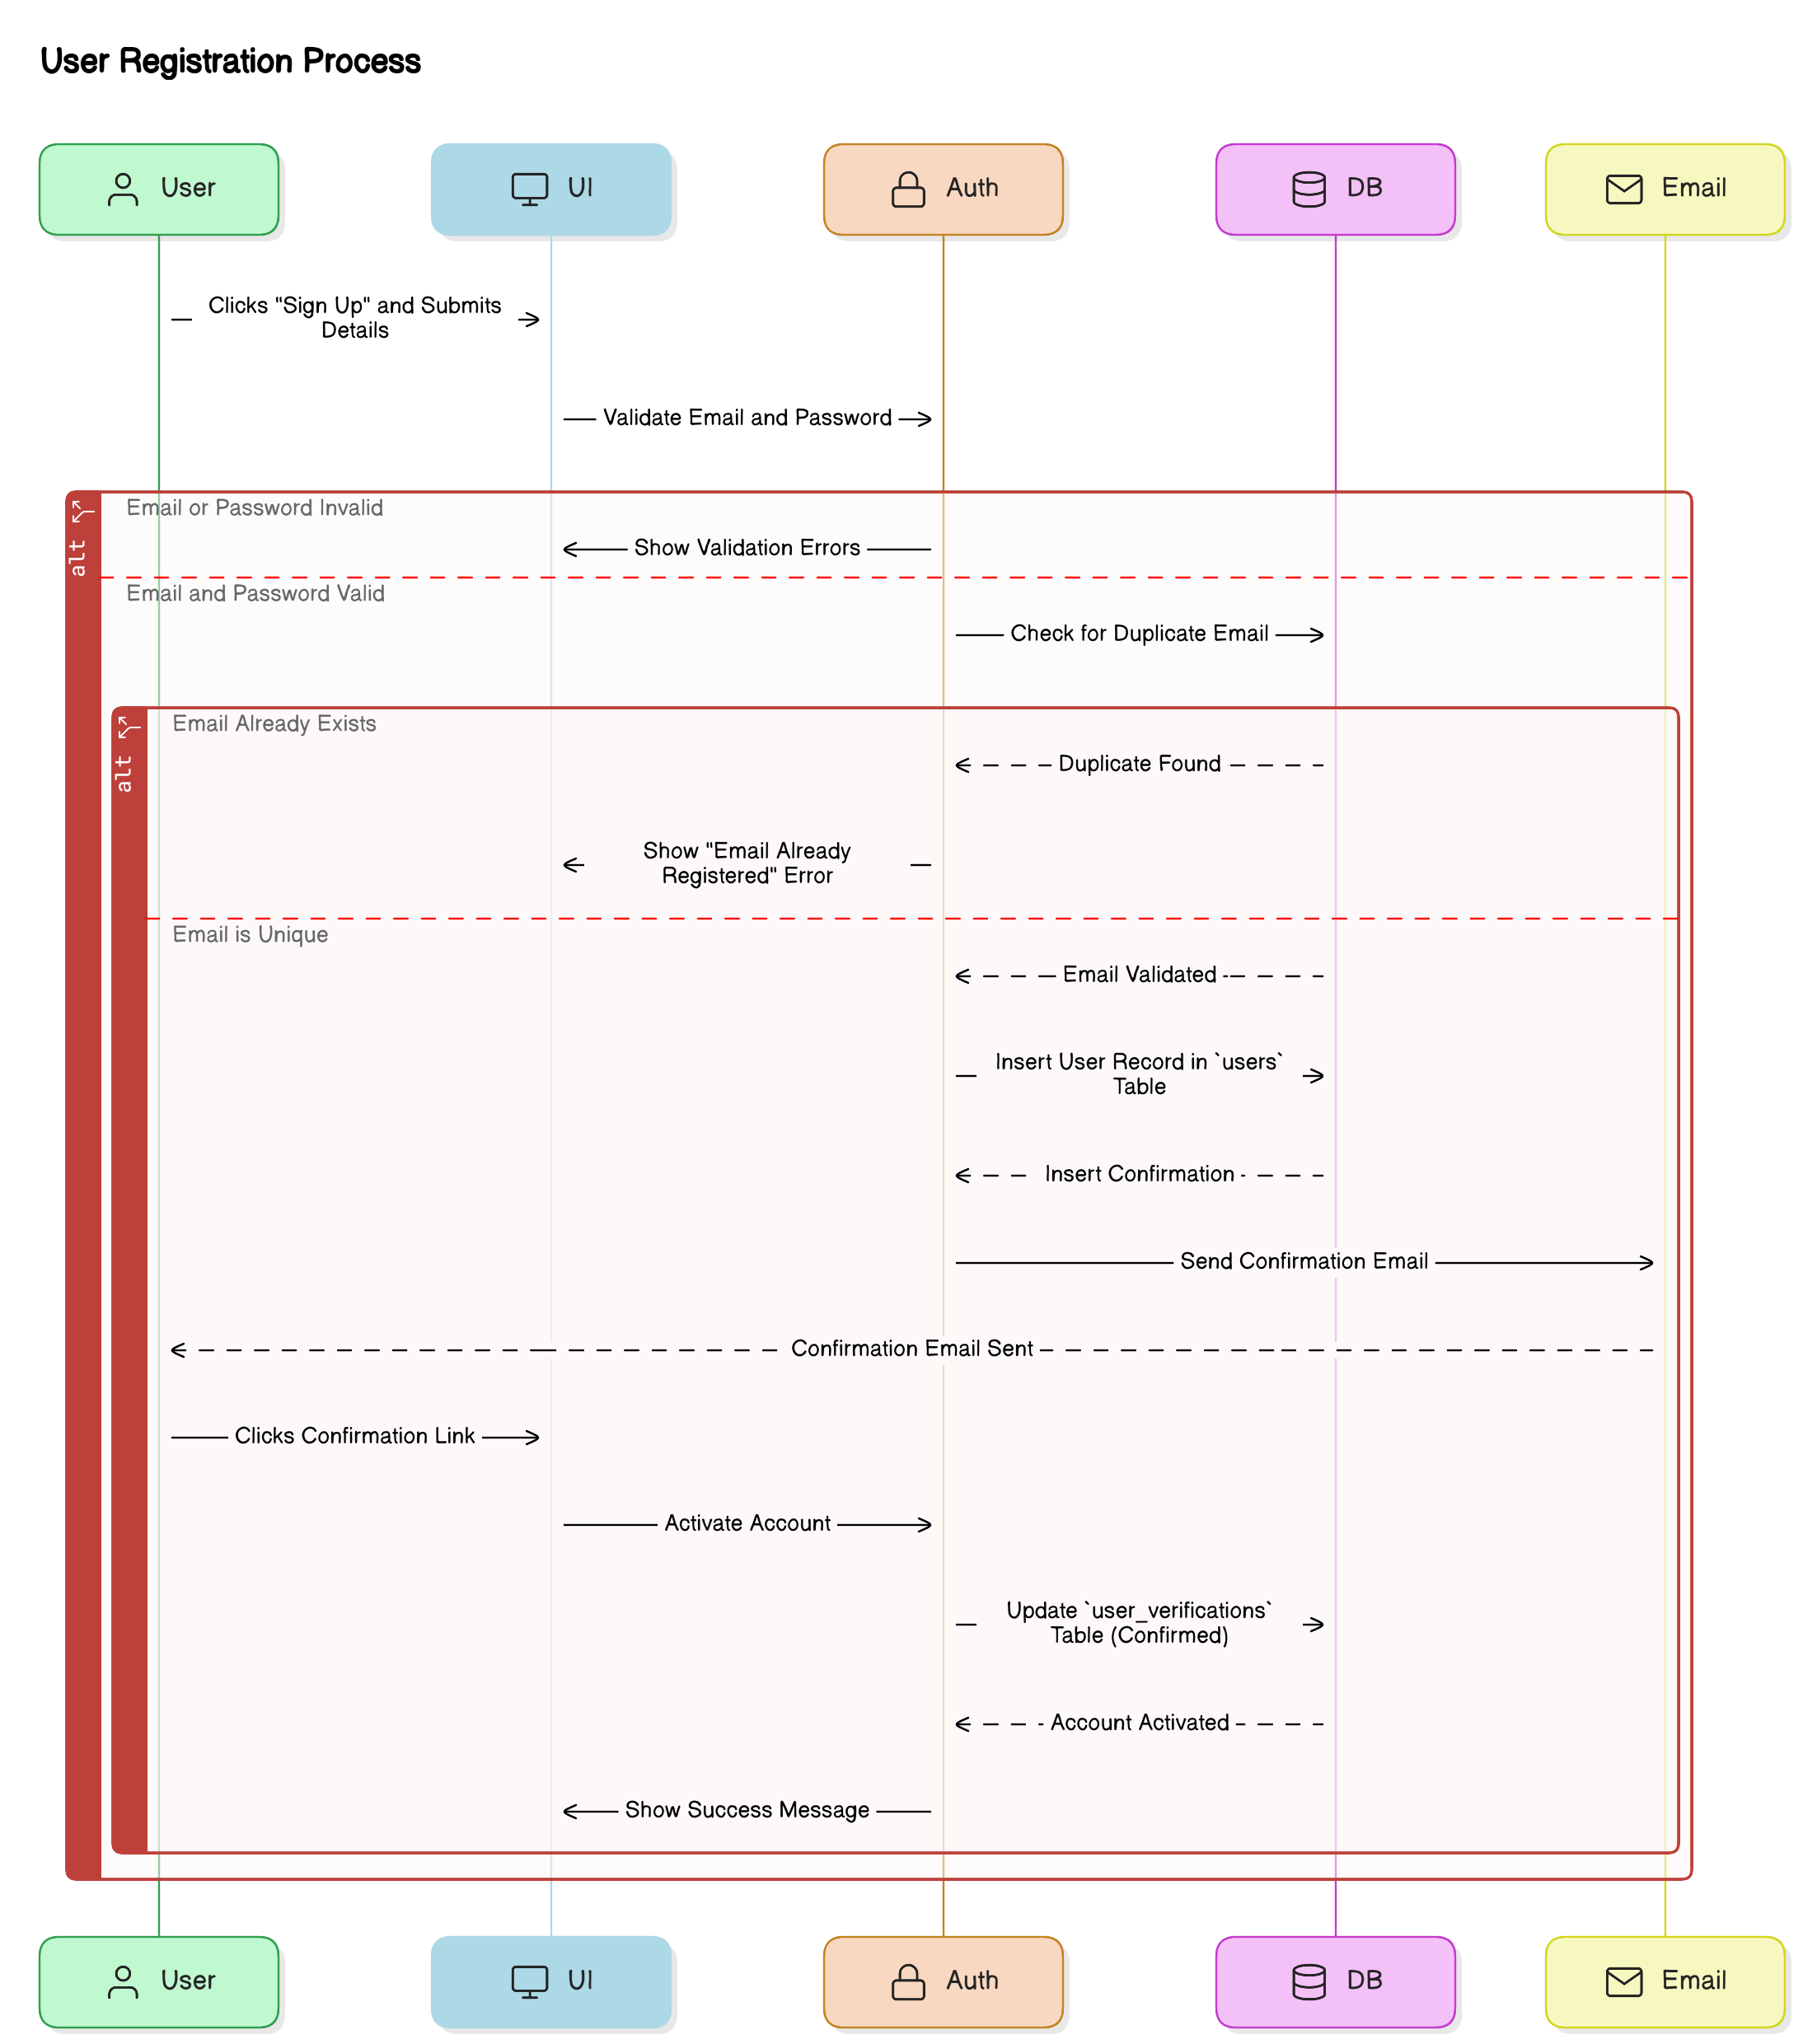
\includegraphics[width=0.9\textwidth]{images/sequence_diagrams/user_registration_process.png}
    \caption{User registration sequence diagram}
    \label{fig:user_registration}
\end{figure}

\subsection{User Login Process}
\begin{figure}[H]
    \centering
    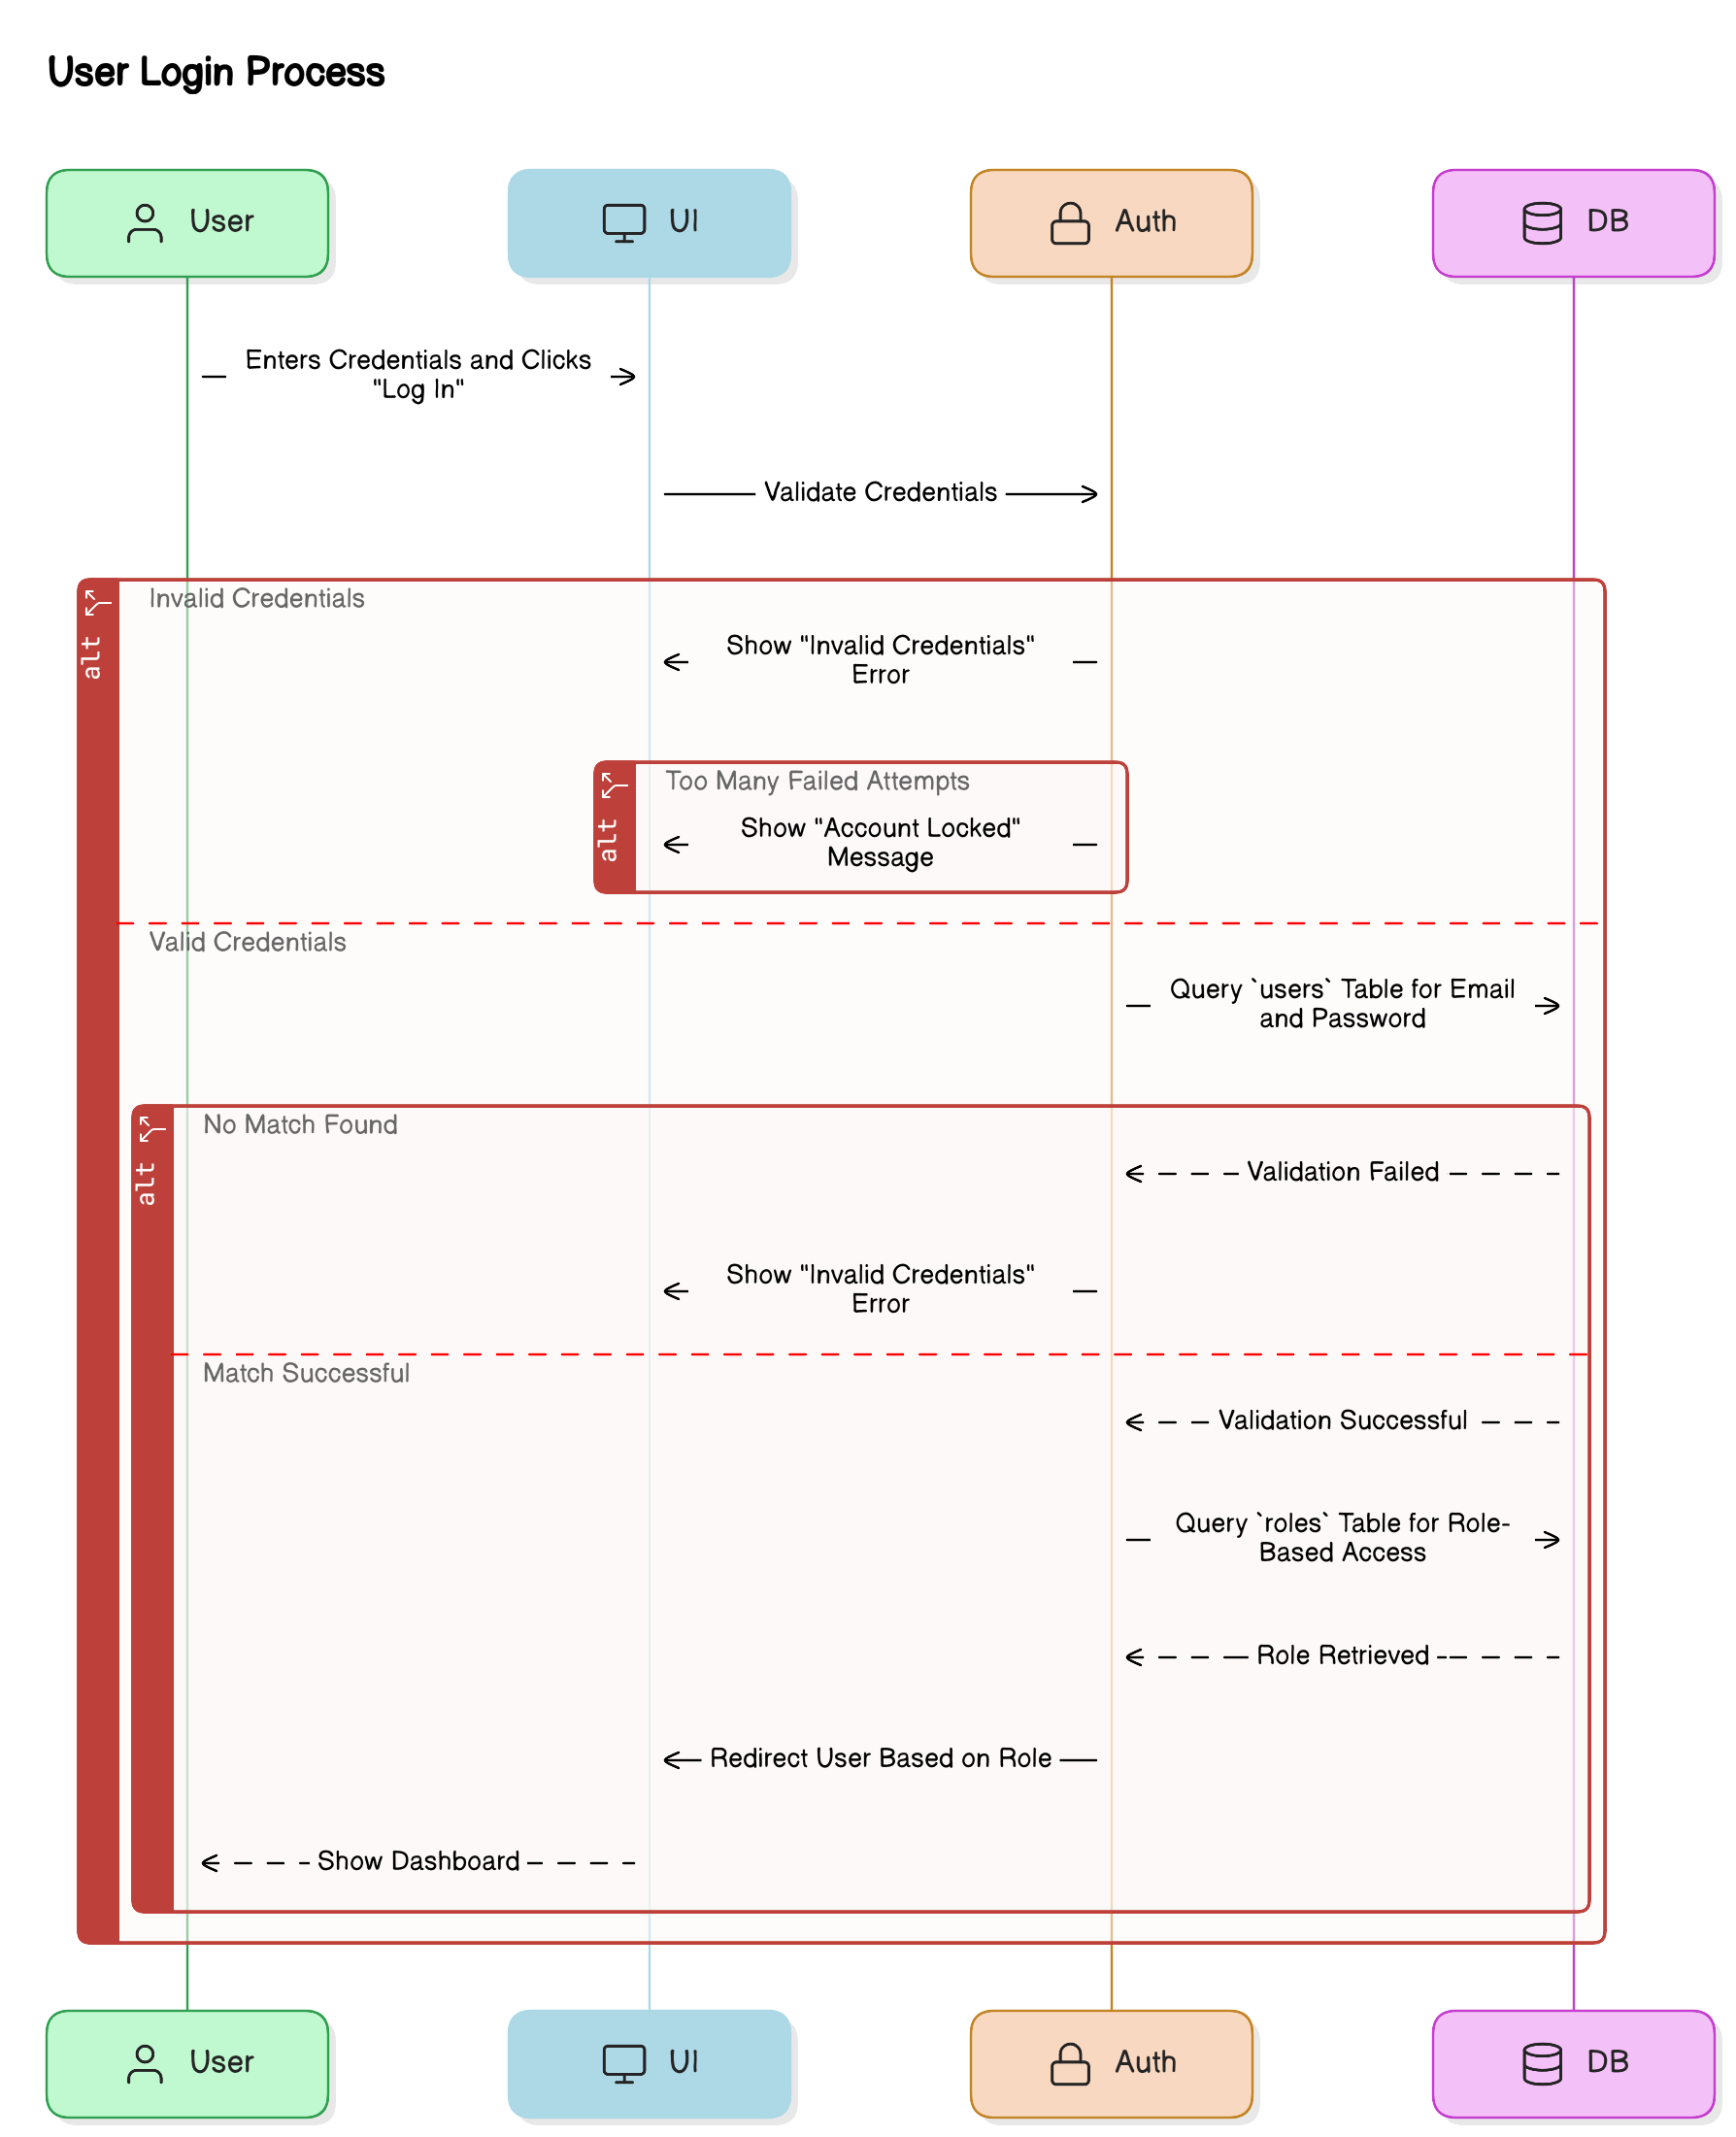
\includegraphics[width=0.9\textwidth]{latex-doc/images/sequence_diagrams/user_login_process.png}
    \caption{Authentication sequence with security measures}
    \label{fig:user_login}
\end{figure}

\subsection{Password Recovery Process}
\begin{figure}[H]
    \centering
    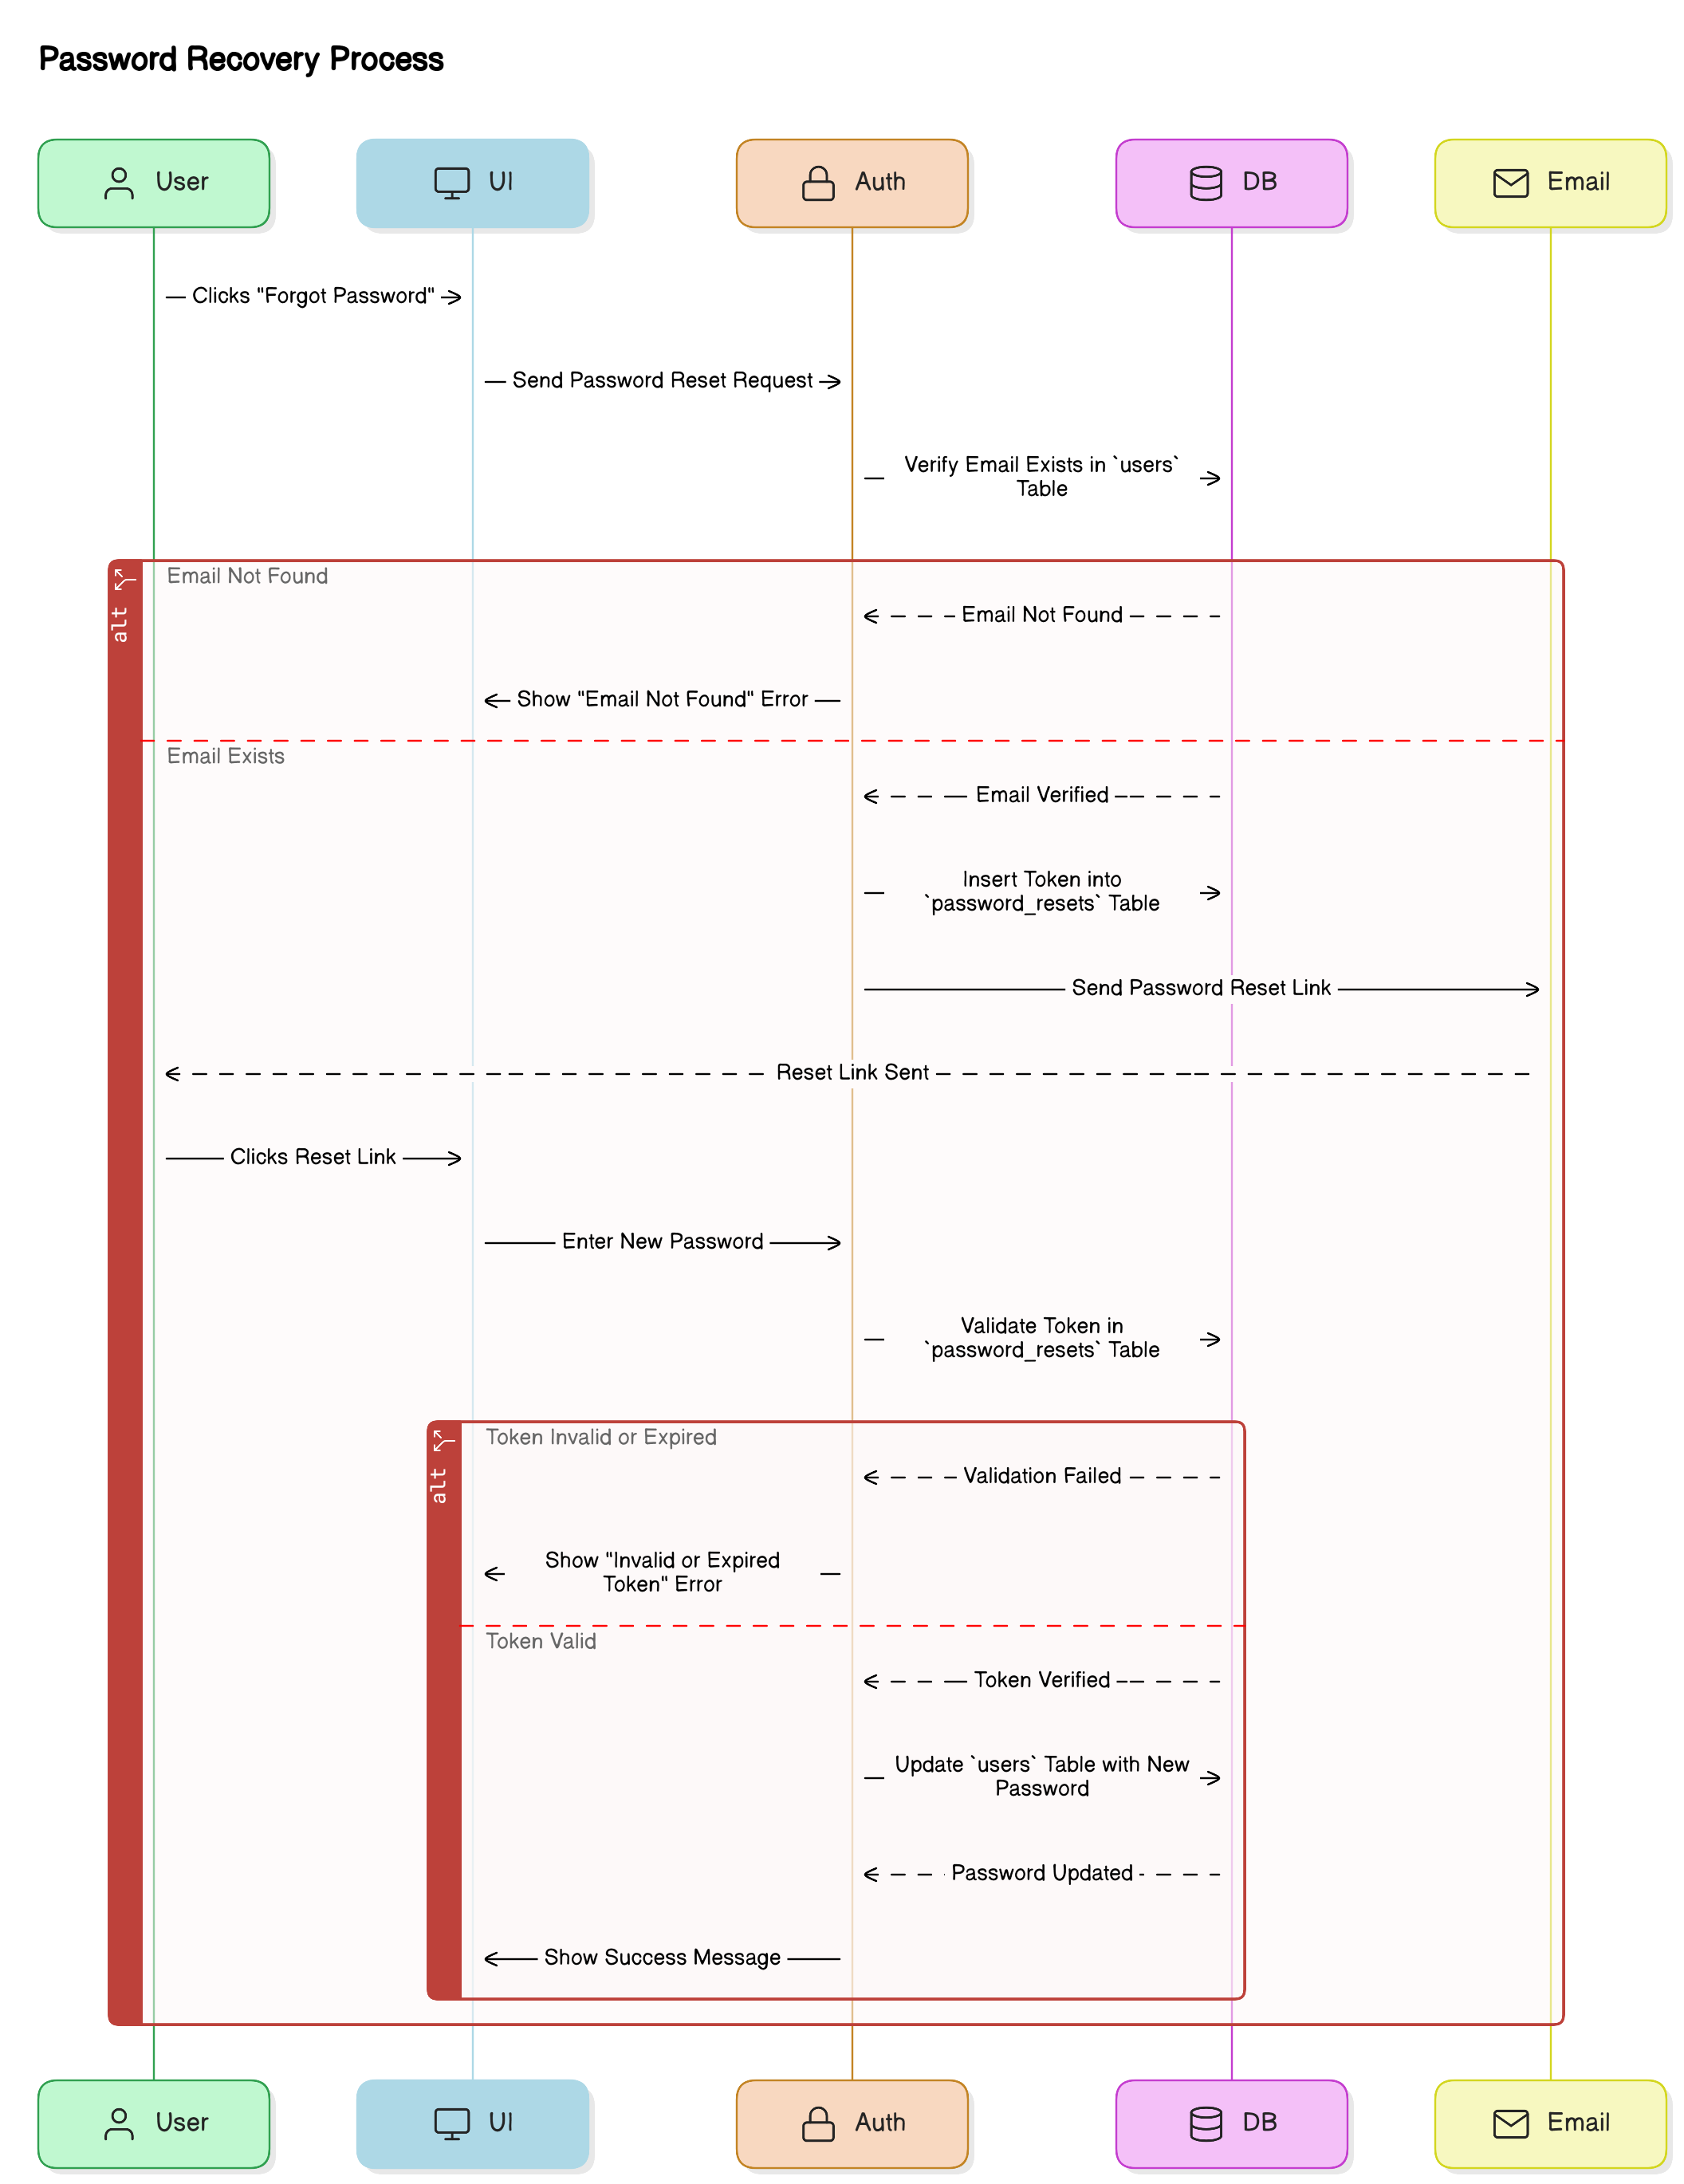
\includegraphics[width=0.9\textwidth]{latex-doc/images/sequence_diagrams/password_recovery_process.png}
    \caption{Password reset sequence diagram with email verification}
    \label{fig:password_recovery}
\end{figure}

\subsection{Create Profile Process}
\begin{figure}[H]
    \centering
    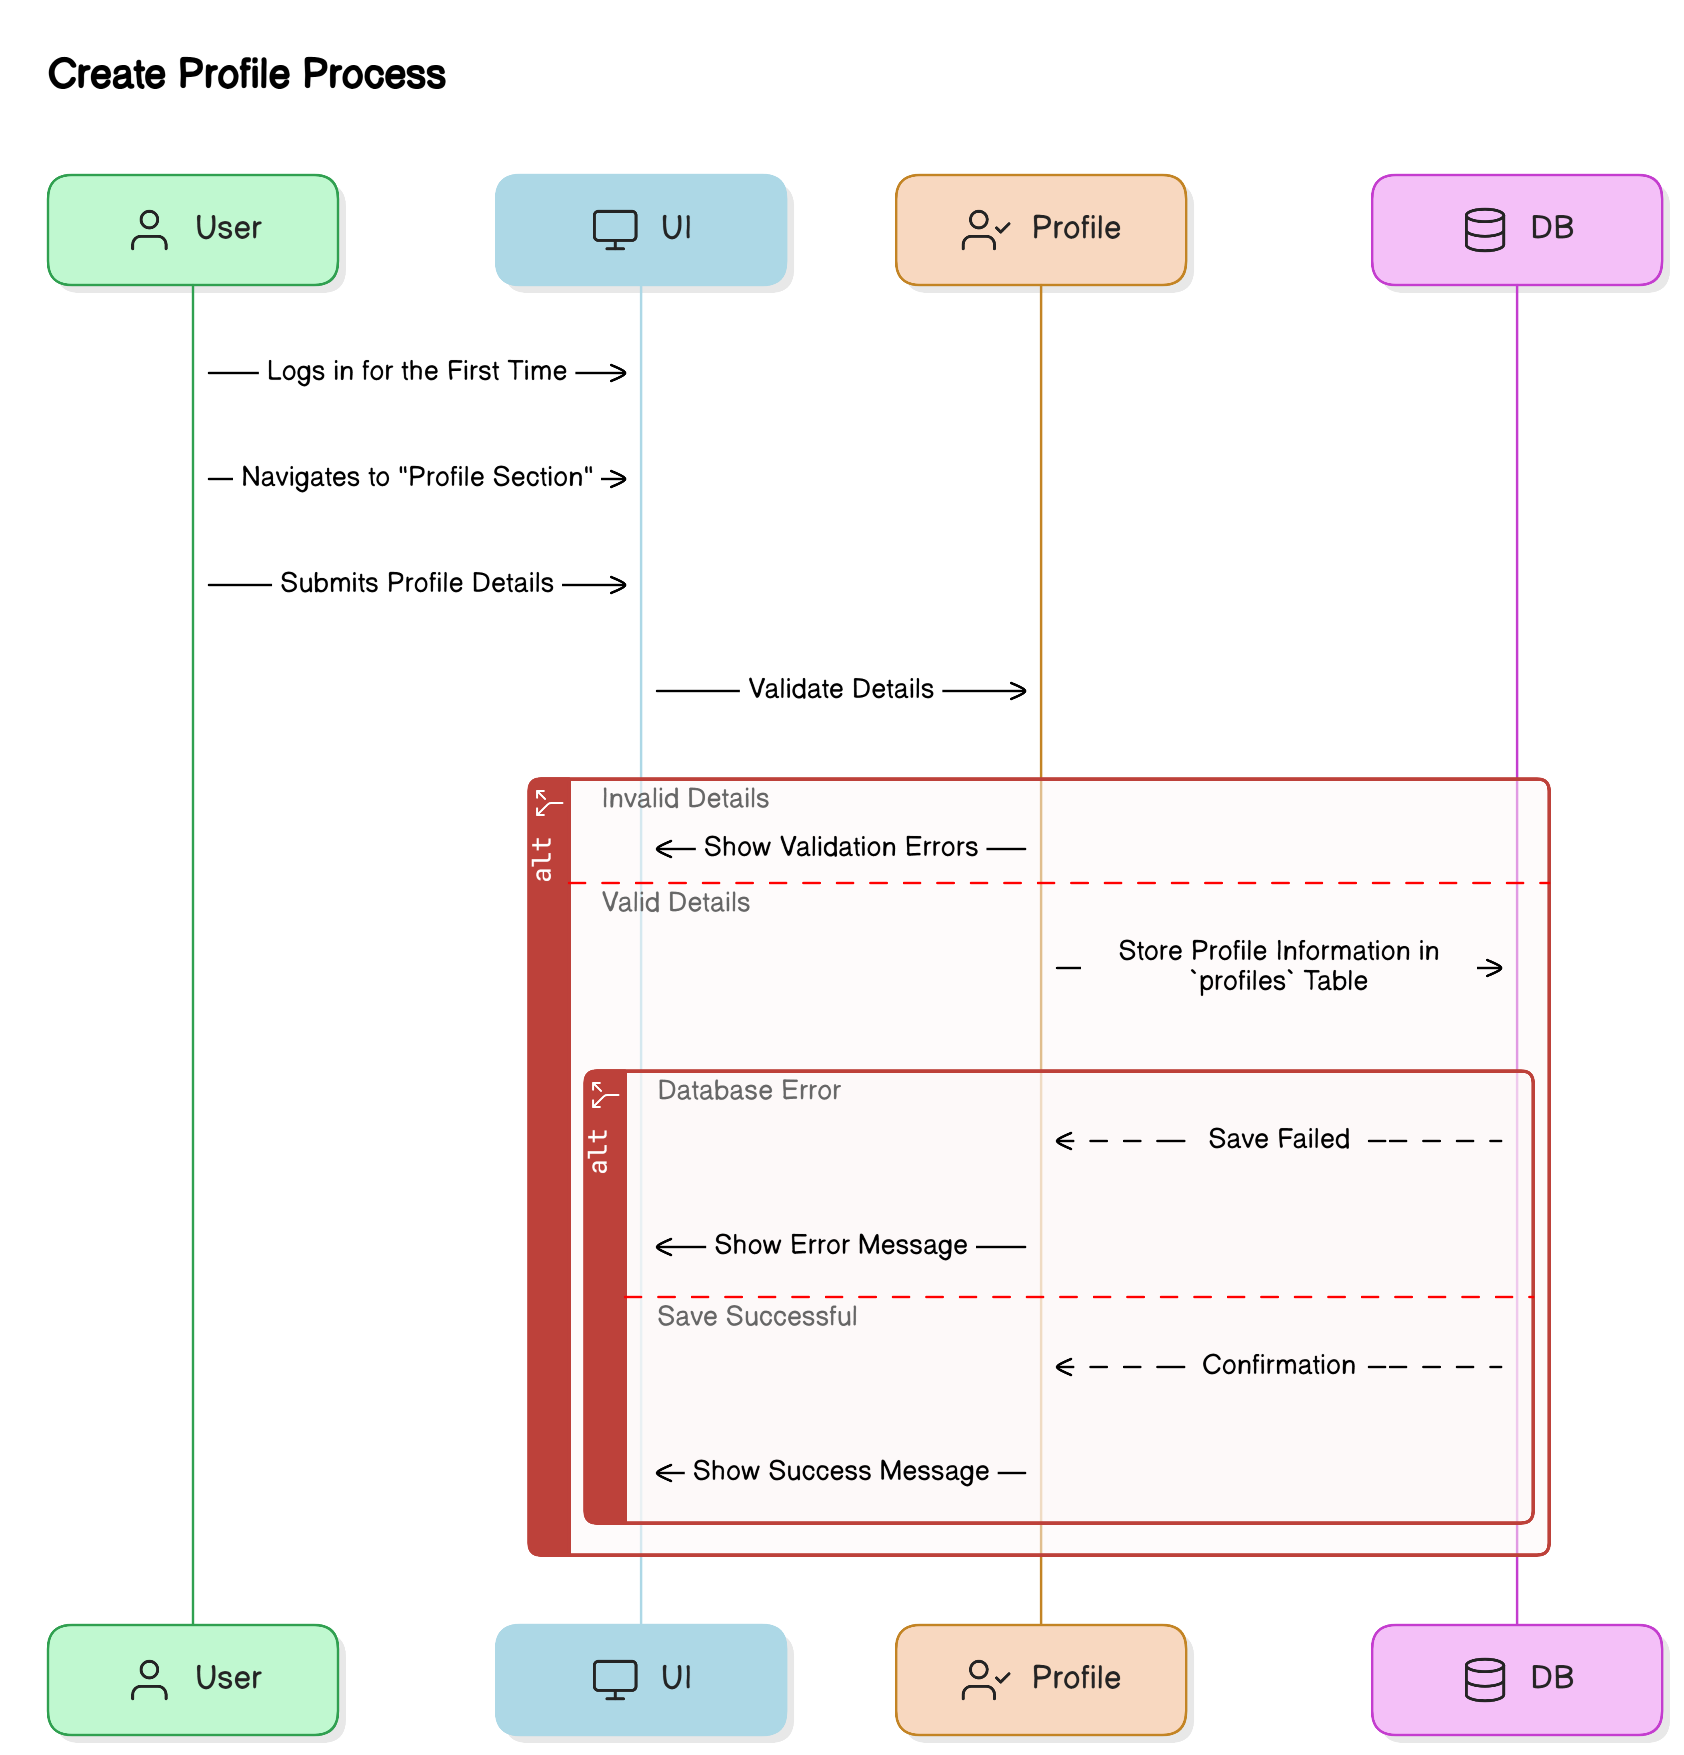
\includegraphics[width=0.9\textwidth]{latex-doc/images/sequence_diagrams/create_profile_process.png}
    \caption{Profile creation sequence diagram showing validation and database storage}
    \label{fig:create_profile}
\end{figure}

\subsection{Create Group Process}
\begin{figure}[H]
    \centering
    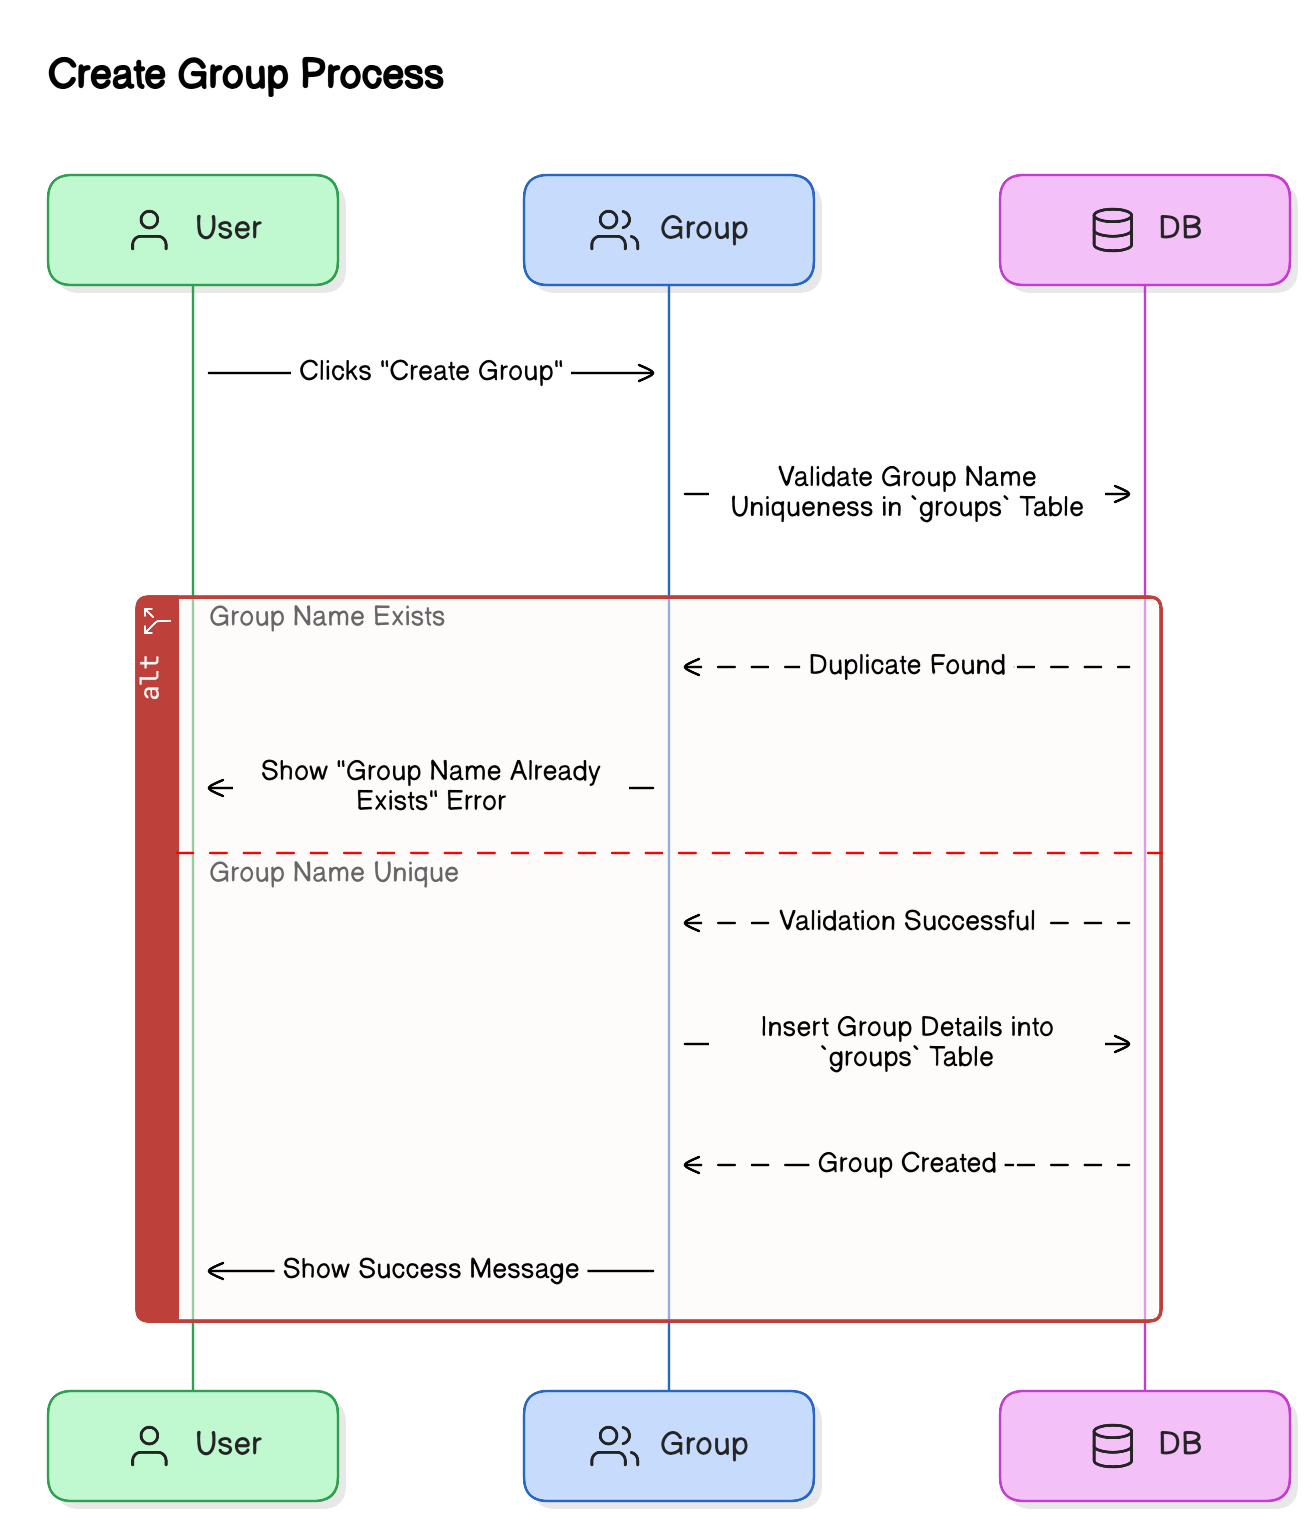
\includegraphics[width=0.9\textwidth]{latex-doc/images/sequence_diagrams/create_group_process.png}
    \caption{Group creation sequence diagram}
    \label{fig:create_group}
\end{figure}

\subsection{Direct Messaging Process}
\begin{figure}[H]
    \centering
    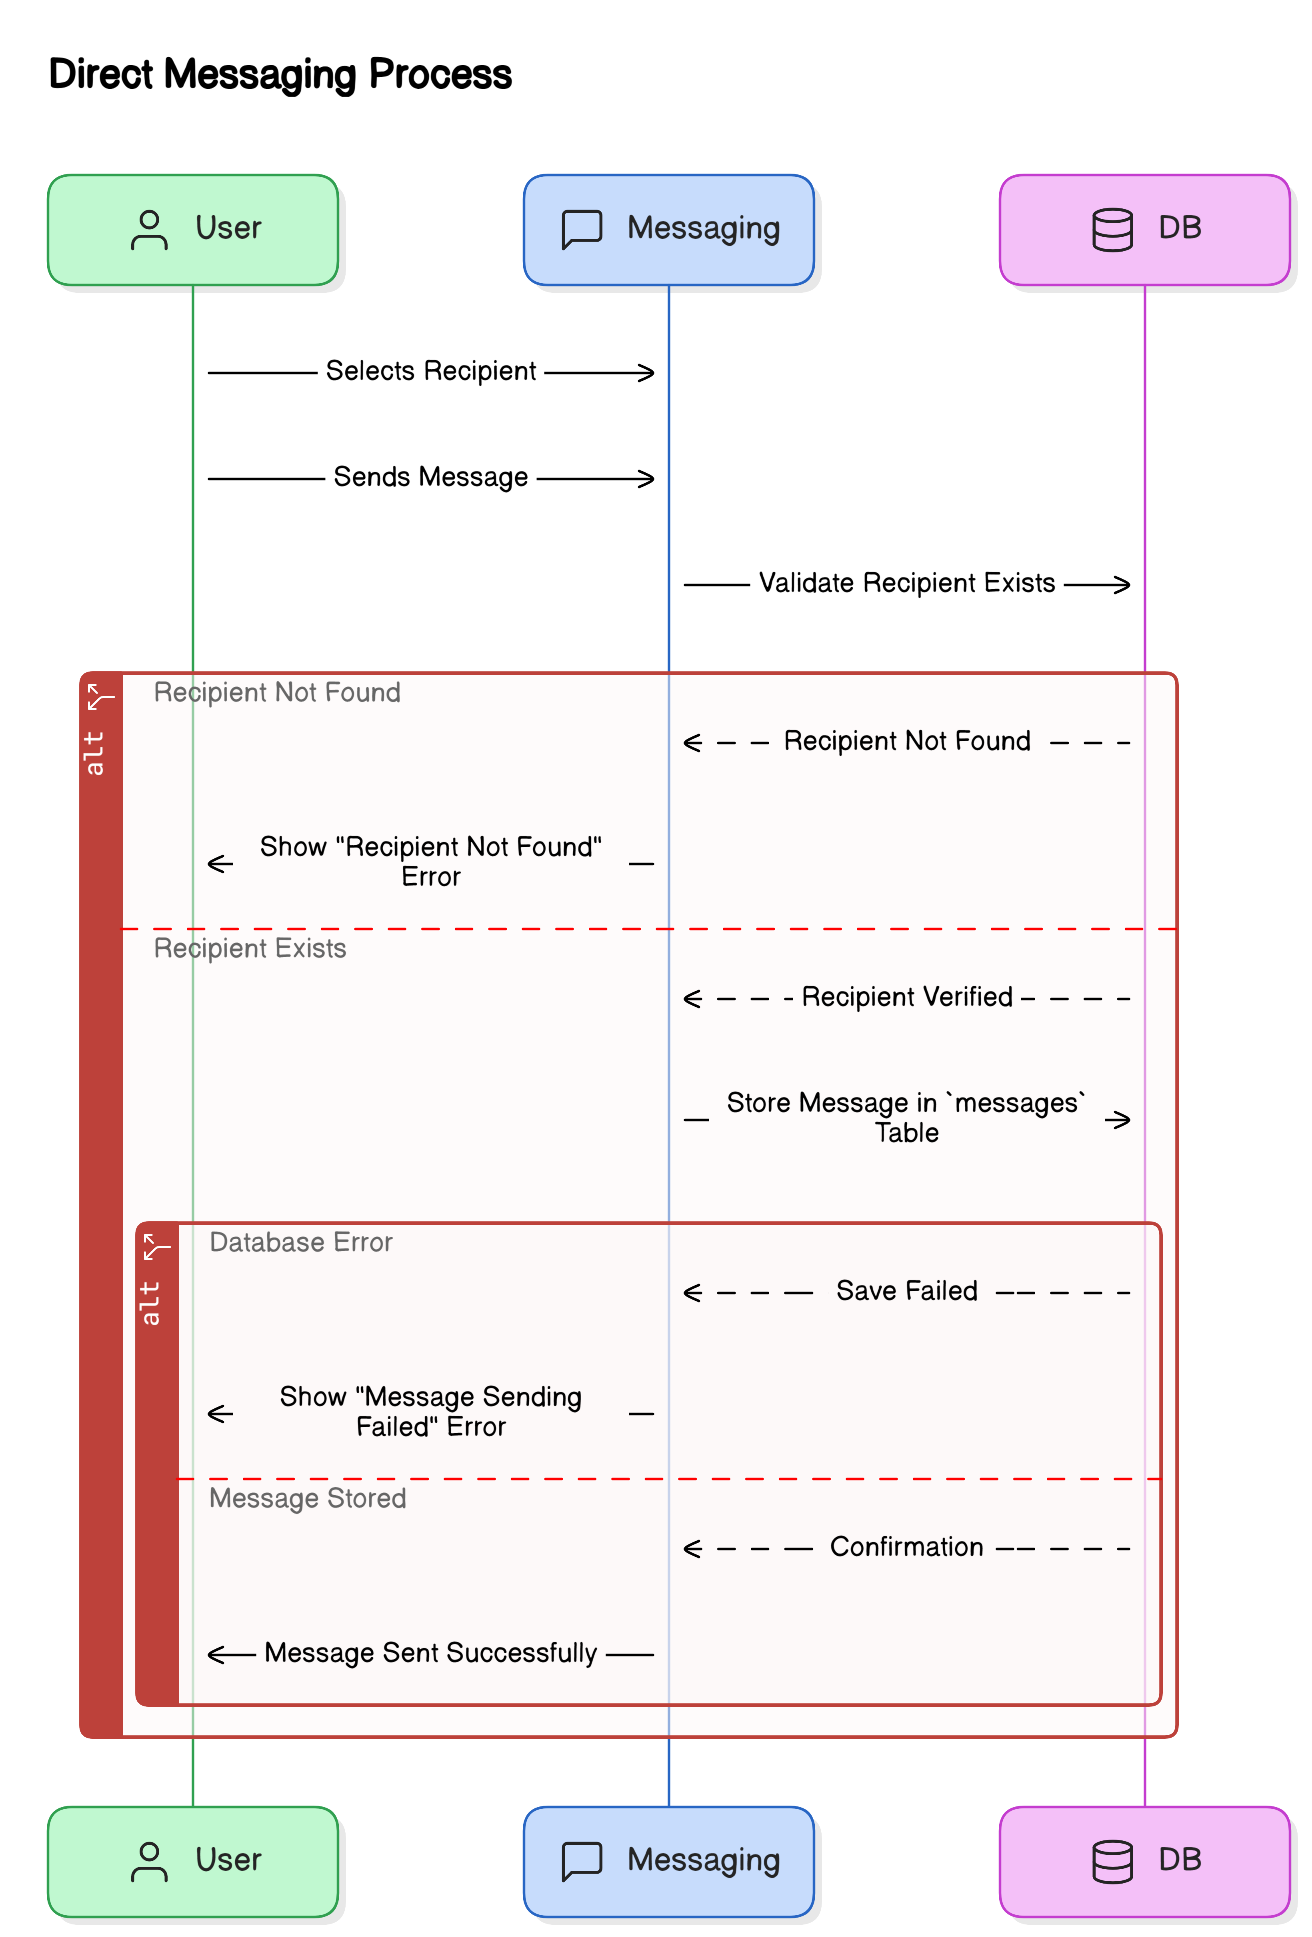
\includegraphics[width=0.9\textwidth]{latex-doc/images/sequence_diagrams/direct_messaging_process.png}
    \caption{Messaging sequence diagram}
    \label{fig:messaging}
\end{figure}

\subsection{Start a Discussion Process}
\begin{figure}[H]
    \centering
    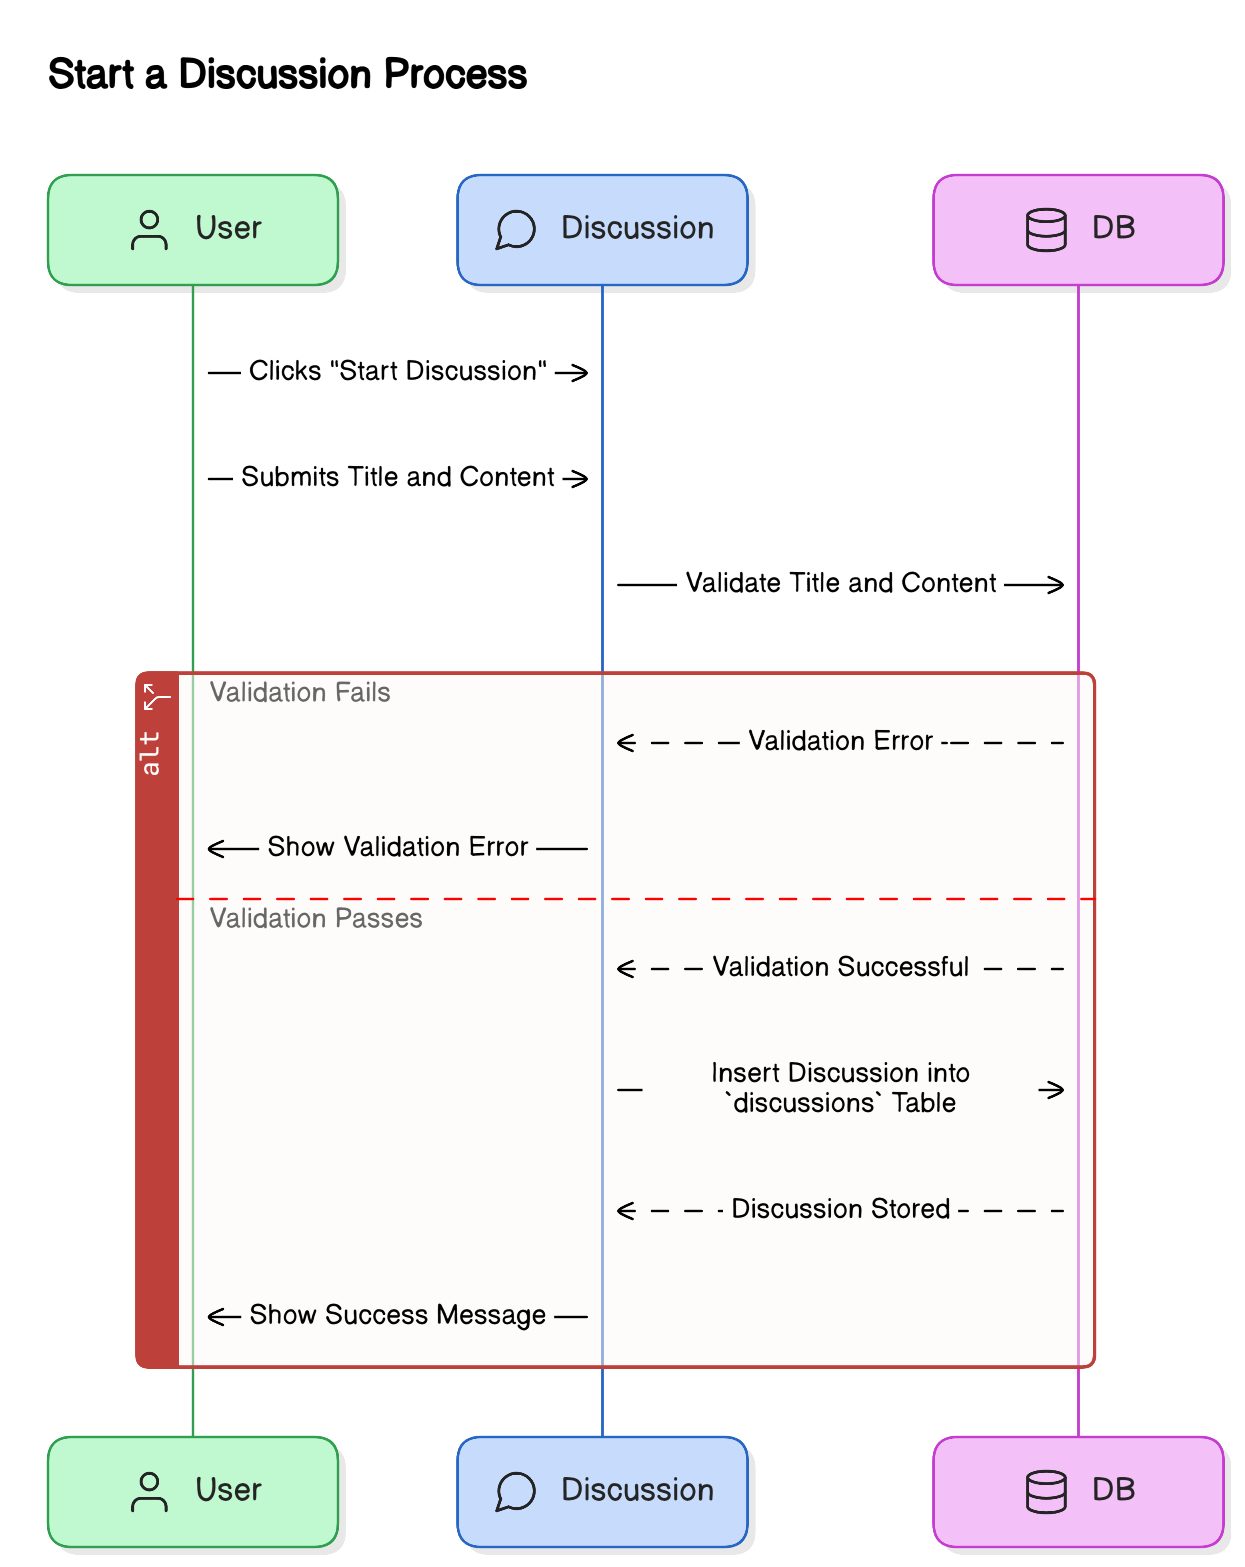
\includegraphics[width=0.9\textwidth]{latex-doc/images/sequence_diagrams/start_a_discussion_process.png}
    \caption{Group discussion initiation sequence}
    \label{fig:start_discussion}
\end{figure}

\subsection{Upload Academic Material Process}
\begin{figure}[H]
    \centering
    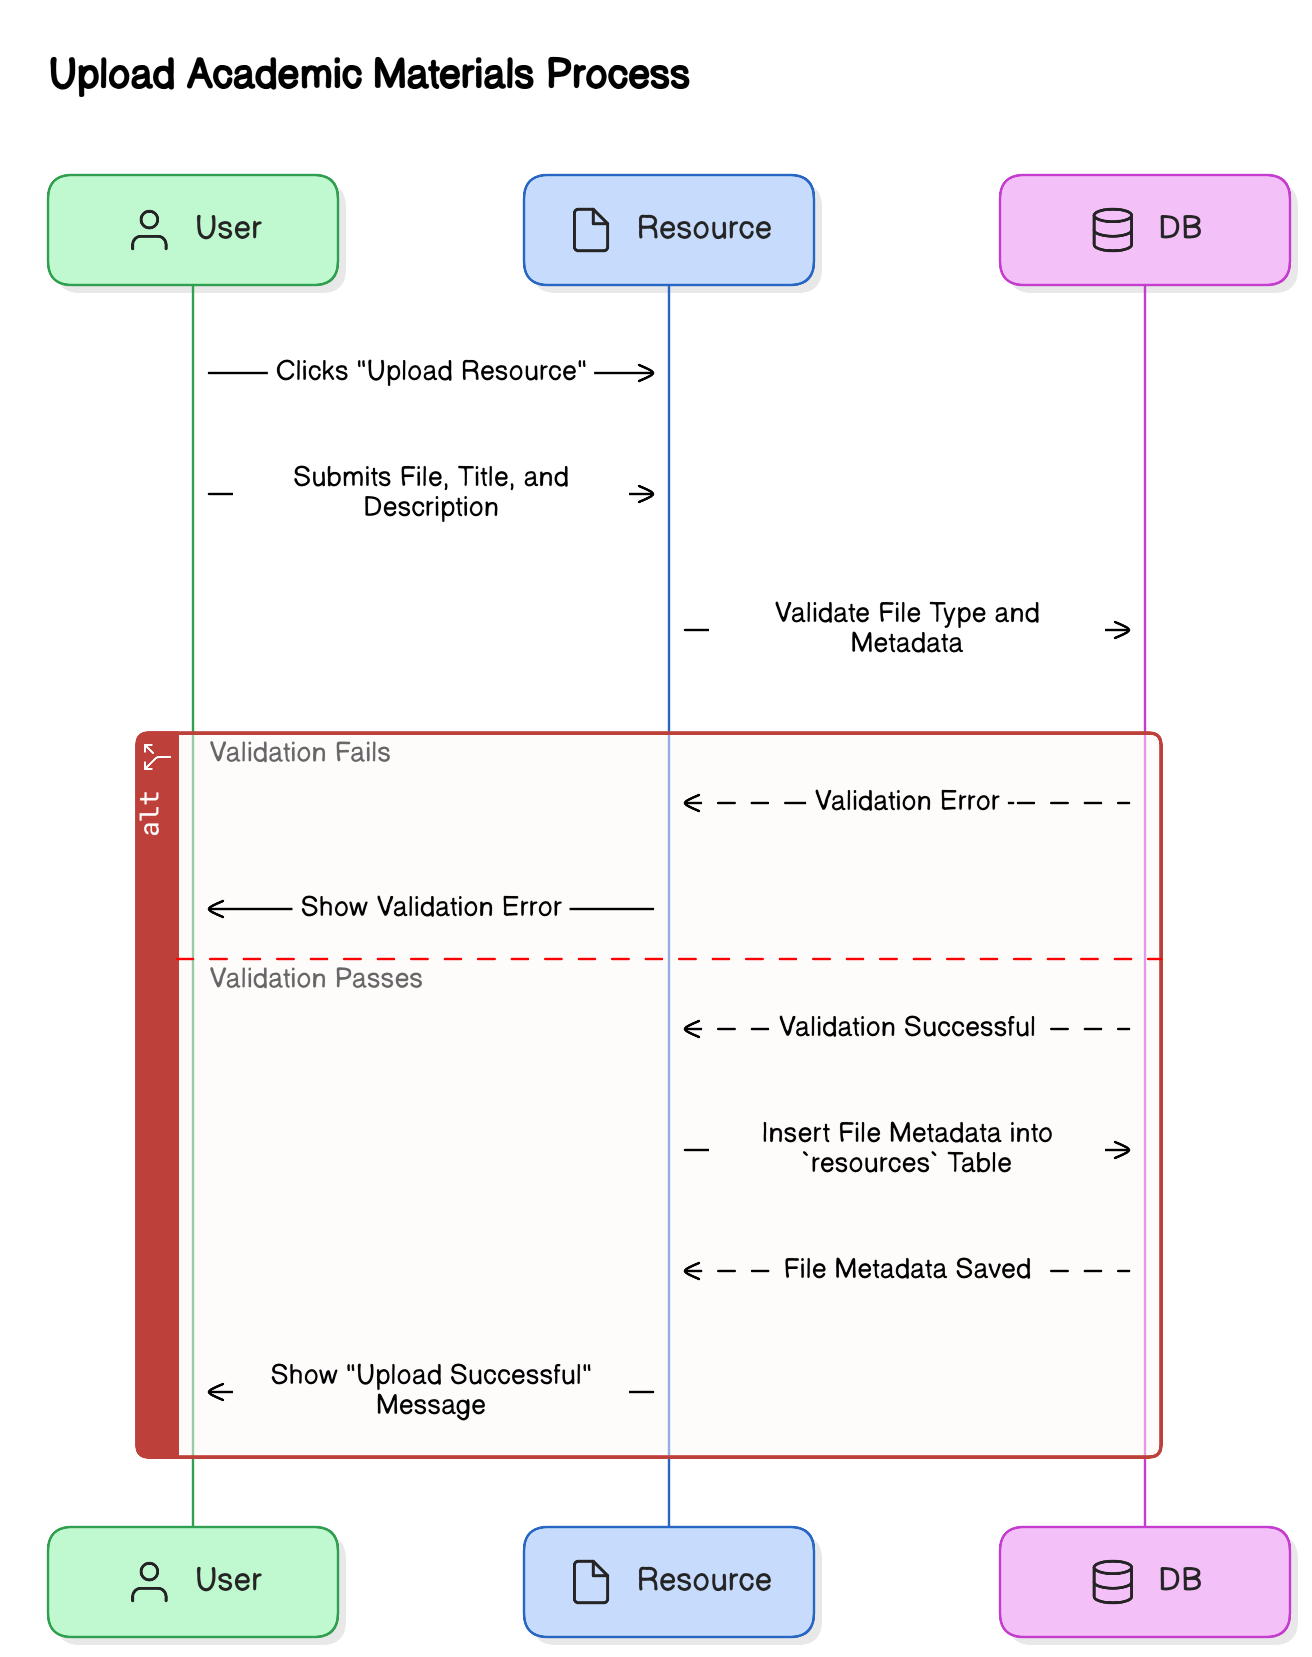
\includegraphics[width=0.9\textwidth]{latex-doc/images/sequence_diagrams/upload_academic_material_process.png}
    \caption{Resource upload sequence with file validation}
    \label{fig:upload_material}
\end{figure}

\subsection{Create Event Process}
\begin{figure}[H]
    \centering
    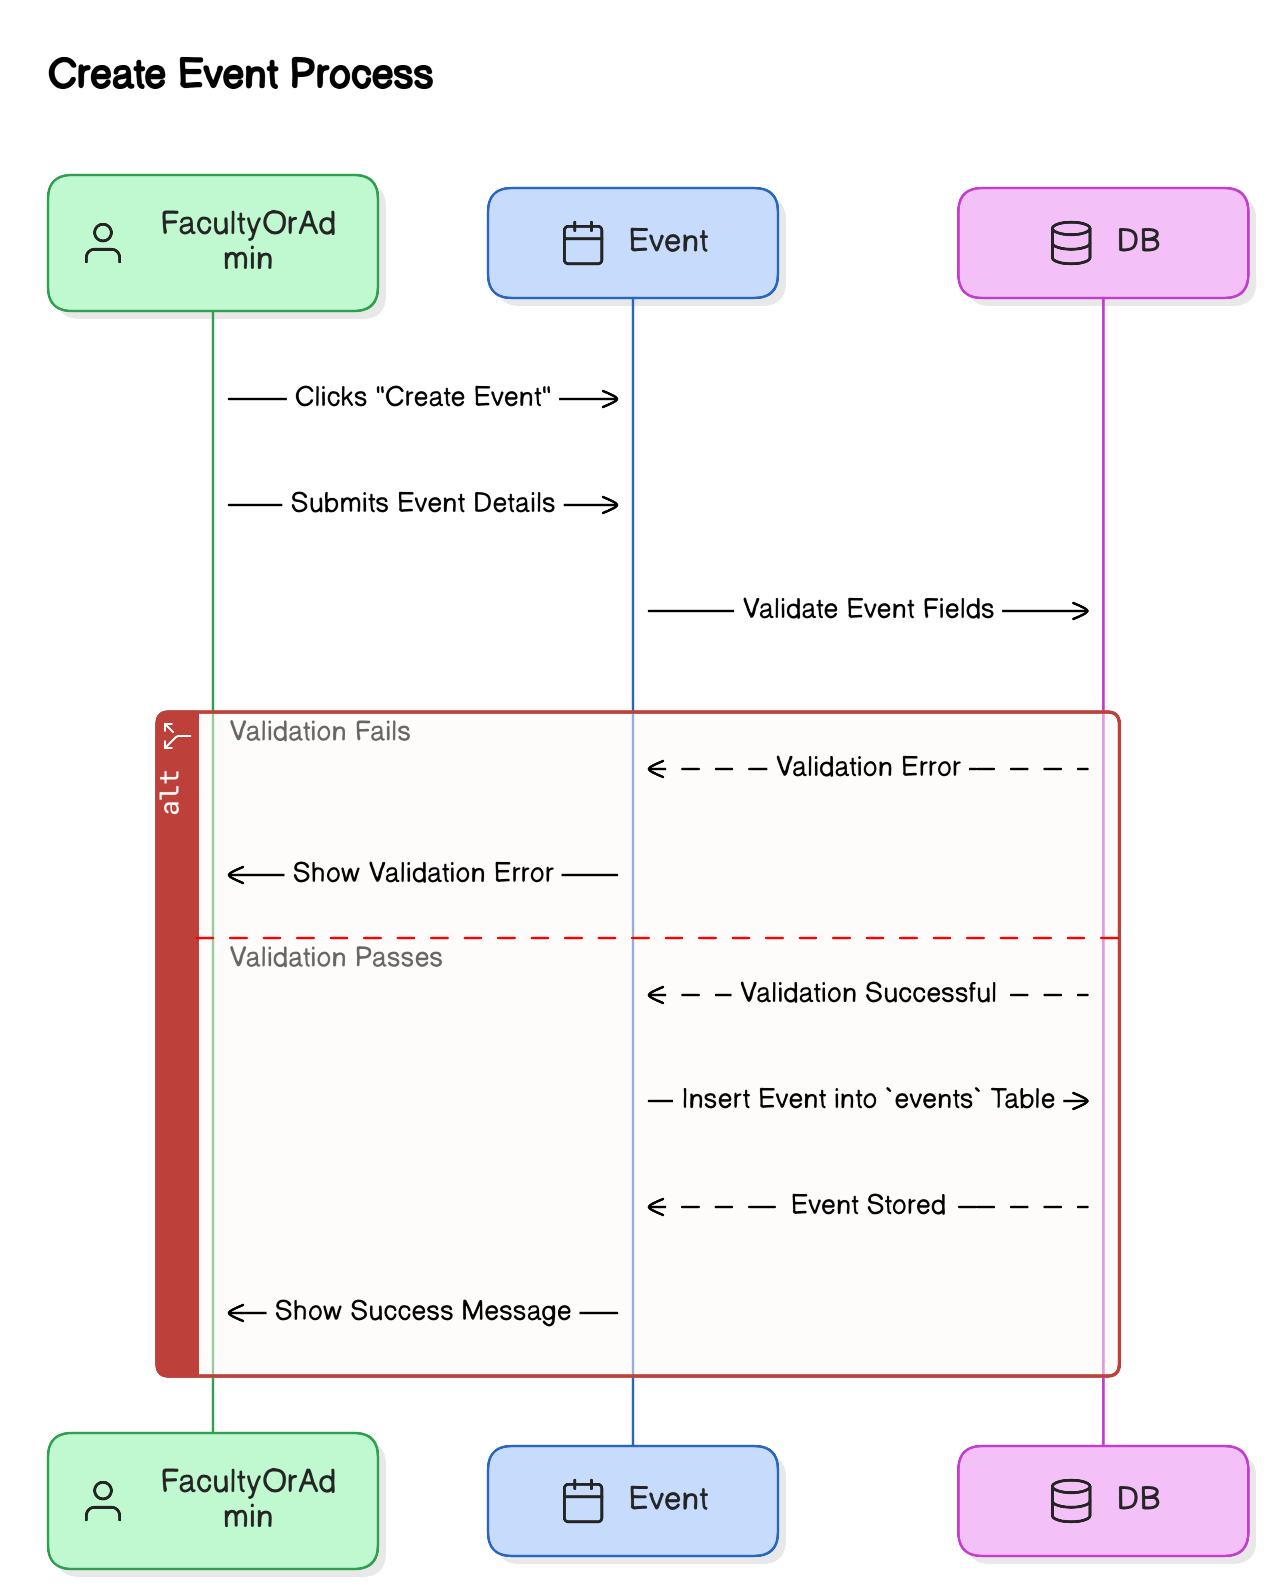
\includegraphics[width=0.9\textwidth]{latex-doc/images/sequence_diagrams/create_event_process.png}
    \caption{Event creation workflow for faculty/admins}
    \label{fig:create_event}
\end{figure}

\vspace{3cm}

\section{Class Diagram}
The class diagram represents the core domain model of the Student Portal system:

\begin{figure}[H]
    \centering
    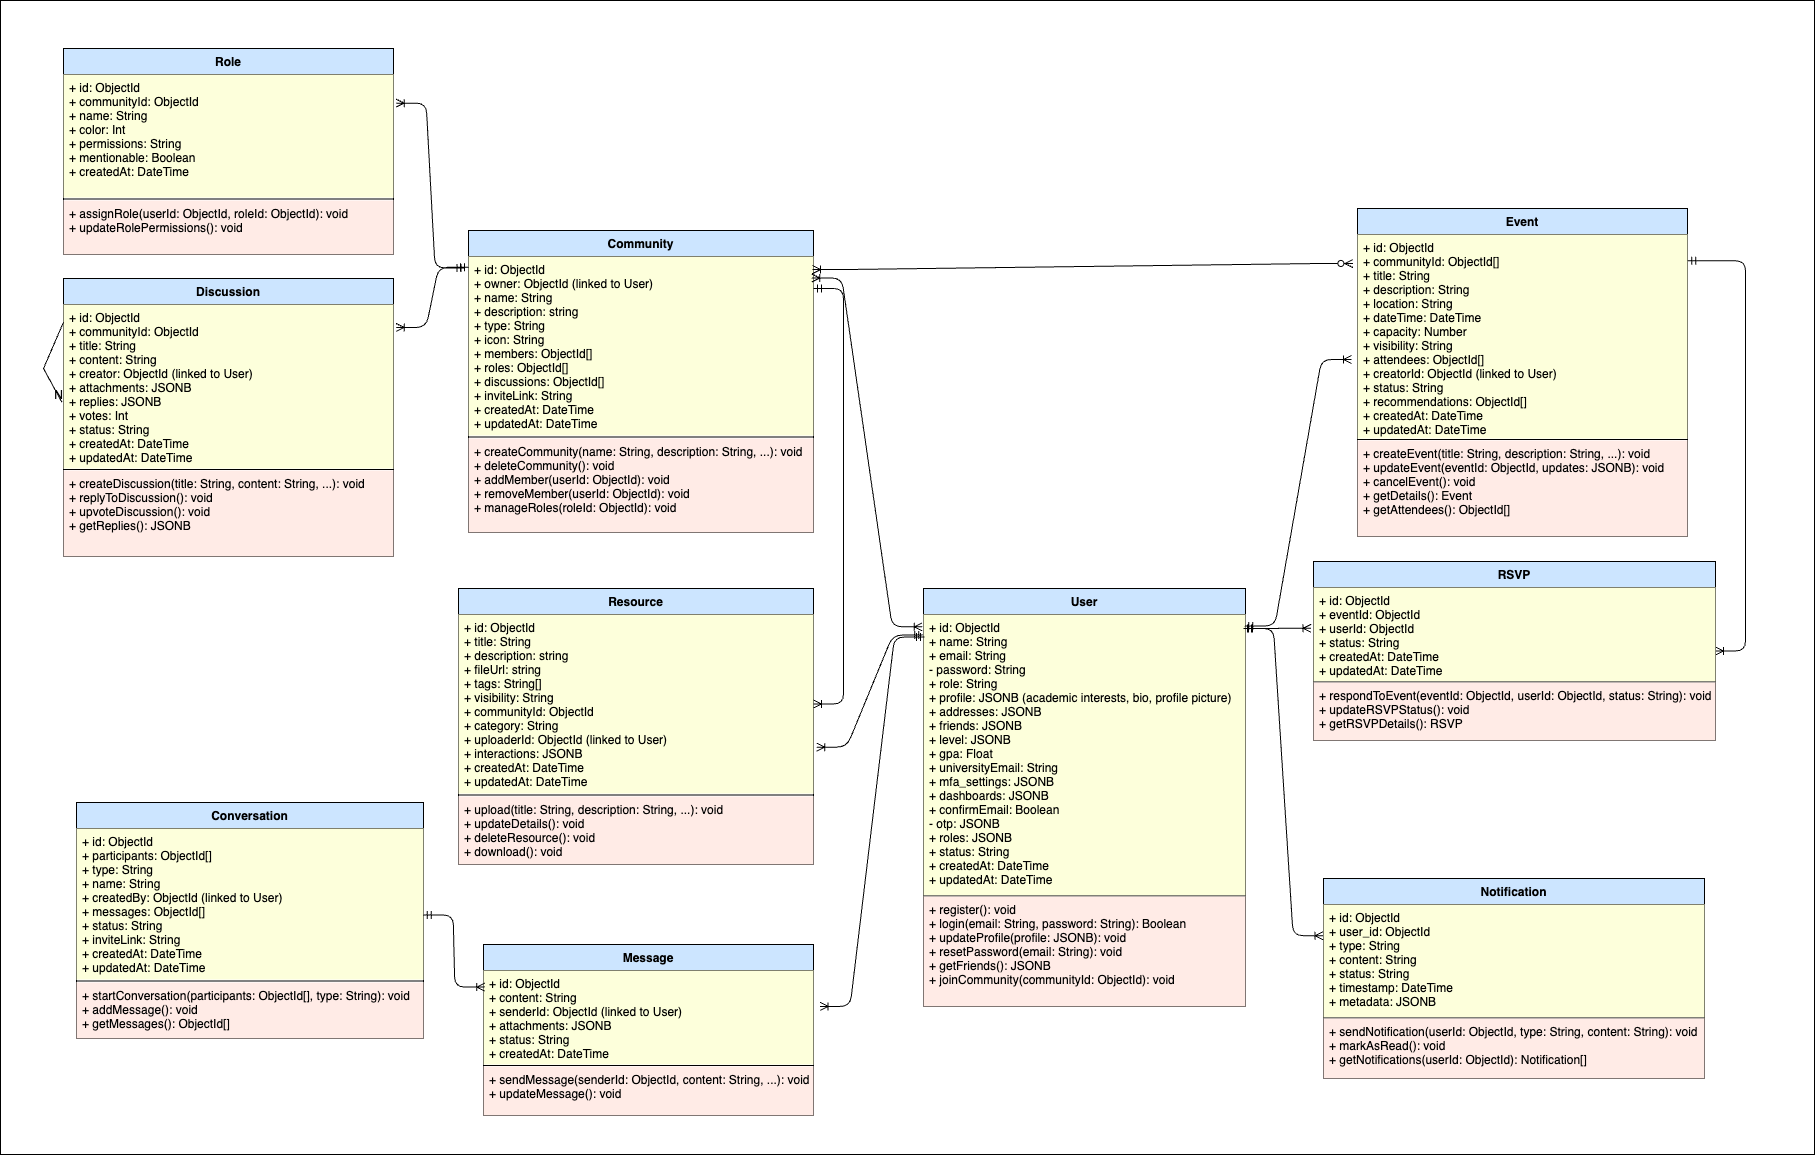
\includegraphics[width=\textwidth]{latex-doc/images/uml.png} 
    \caption{Class diagram of the Student Portal system}
    \label{fig:class_diagram}
\end{figure}

\section{Entity Relationship Diagram (ERD)}
\begin{adjustbox}{width=\textwidth, height=0.35\textheight, keepaspectratio, center}
    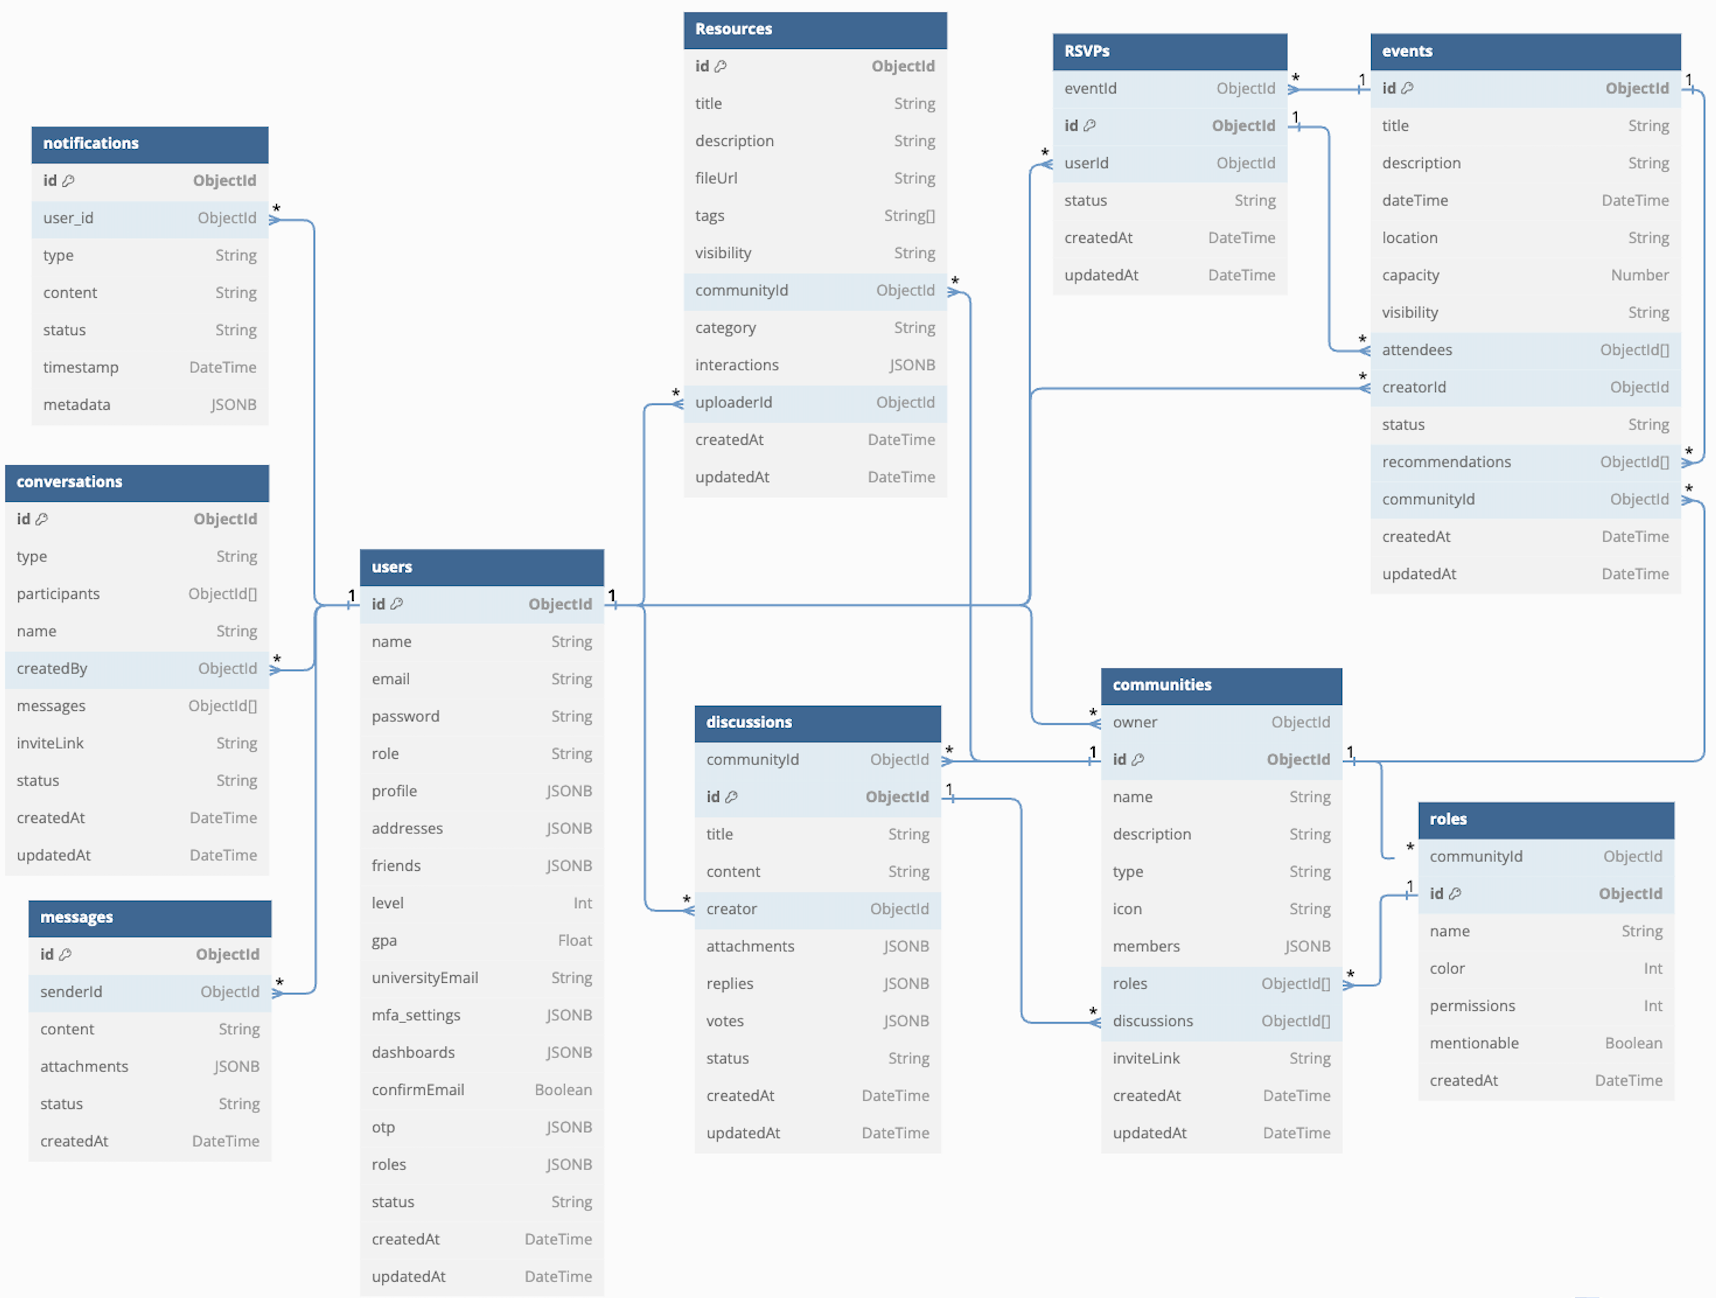
\includegraphics{latex-doc/images/schema_diagram.png}
\end{adjustbox}



\section{Data Dictionary}

\subsection{Users Table}
\begin{longtable}{|L{3cm}|C{2cm}|L{2.5cm}|L{3cm}|L{3cm}|}
\hline
\textbf{Field} & \textbf{Type} & \textbf{Description} & \textbf{Constraints} & \textbf{Example} \\ \hline
\endhead

id & ObjectId & Unique user identifier & Primary key, auto-generated & 507f1f77bc-f86cd799439011 \\ \hline
name & String & Full name of the user & Required, max 255 chars & John Doe \\ \hline
email & String & Login credential & Unique, required & john.doe@ example.com \\ \hline
password & String & Encrypted password & Bcrypt hashed & hashed\_password \\ \hline
role & String & Access level & Enum: Student/Faculty/Admin & Student \\ \hline
profile & JSONB & User profile data & Optional & \{bio:CS Student\} \\ \hline
status & String & Online status & Enum: online/offline/ idle/dnd & online \\ \hline
createdAt & DateTime & Account creation time & Auto-generated & 2023-07-01T12:00:00Z \\ \hline

\caption{Users table data dictionary}
\label{tab:users_dict}
\end{longtable}

\subsection{Communities Table}
\begin{longtable}{|L{3cm}|C{2cm}|L{2.5cm}|L{3cm}|L{3cm}|}
\hline
\textbf{Field} & \textbf{Type} & \textbf{Description} & \textbf{Constraints} & \textbf{Example} \\ \hline
\endhead

id & ObjectId & Group identifier & Primary key, auto-generated & 507f1f77bc-f86cd799439200 \\ \hline
name & String & Community name & Unique, required & AI Enthusiasts \\ \hline
type & String & Group classification & Enum: official/community & official \\ \hline
owner & ObjectId & Creator reference & Foreign key to users & 507f1f77bc-f86cd799439100 \\ \hline
members & JSONB & Member list & Array of user objects & \{userId:507...\} \\ \hline
createdAt & DateTime & Creation timestamp & Auto-generated & 2024-01-10T08:45:00Z \\ \hline

\caption{Communities table data dictionary}
\label{tab:communities_dict}
\end{longtable}

\subsection{Embedded Structures}

\begin{longtable}{|C{3.5cm}|C{2cm}|C{4cm}|C{3cm}|}
\hline
\textbf{Field} & \textbf{Type} & \textbf{Description} & \textbf{Example} \\ \hline
\endhead

members.userId & ObjectId & Member reference & 507f1f77bcf 86cd799439101 \\ \hline
members.roleIds & ObjectId[] & Assigned roles & ["507f1f77bcf8 6cd799439300"] \\ \hline
members.joinedAt & DateTime & Join timestamp & 2024-01-10T09:30:00Z \\ \hline

\caption{Embedded members structure}
\label{tab:members_struct}
\end{longtable}

\subsection{Discussions Table}
\begin{longtable}{|L{3cm}|C{2cm}|L{2.5cm}|L{3cm}|L{3cm}|}
\hline
\textbf{Field} & \textbf{Type} & \textbf{Description} & \textbf{Constraints} & \textbf{Example} \\ \hline
\endhead

id & ObjectId & Discussion identifier & Primary key & 507f1f77bcf8 6cd799439200 \\ \hline
communityId & ObjectId & Parent community & Foreign key & 507f1f77b cf86cd799439100 \\ \hline
title & String & Discussion title & Required, max 255 chars & "Best Practices for Web Dev" \\ \hline
content & String & Main content & Required & "What are the best practices?"  \hline
creator & ObjectId & Author reference & Foreign key to users & 507f1f77bcf 86cd799439101 \hline
status & String & Discussion state & Enum: open/closed/archived & "open" \\ \hline
createdAt & DateTime & Creation time & Auto-generated & 2024-01-10T08: 45:00Z \hline
\caption{Discussions table data dictionary}
\label{tab:discussions_dict}
\end{longtable}

\subsection{Conversations Table}
\begin{longtable}{|L{3cm}|C{2cm}|L{2.5cm}|L{3cm}|L{3cm}|}
\hline
\textbf{Field} & \textbf{Type} & \textbf{Description} & \textbf{Constraints} & \textbf{Example} \\ \hline
\endhead

id & ObjectId & Conversation ID & Primary key & 507f1f77bcf 86cd799439100 \\ \hline
type & String & Conversation type & Enum: DM/GroupDM & "GroupDM" \\ \hline
participants & ObjectId[] & Participant list & Min 2 for GroupDM & ["507...101", "507...102"] \\ \hline
createdBy & ObjectId & Creator reference & Foreign key to users & 507f1f77bc f86cd799439103 \\ \hline
status & String & Conversation state & Enum: active/archived & "active" \\ \hline

\caption{Conversations table data dictionary}
\label{tab:conversations_dict}
\end{longtable}

\subsection{Messages Table}
\begin{longtable}{|L{3cm}|C{2cm}|L{2.5cm}|L{3cm}|L{3cm}|}
\hline
\textbf{Field} & \textbf{Type} & \textbf{Description} & \textbf{Constraints} & \textbf{Example} \\ \hline
\endhead

id & ObjectId & Message identifier & Primary key & 60d21b4667d 0d8992e610c85 \\ \hline
senderId & ObjectId & Sender reference & Foreign key to users & 60d21b4667d 0d8992e610c90 \\ \hline
content & String & Message text & Optional & "Hello, how are you?" \\ \hline
status & String & Delivery status & Enum: sent/ delivered/read & "delivered" \\ \hline
createdAt & DateTime & Send timestamp & Auto-generated & 2024-01-28T12:00:00Z \\ \hline

\caption{Messages table data dictionary}
\label{tab:messages_dict}
\end{longtable}

\subsection{Embedded Structures}

\subsubsection{Discussion Attachments}
\begin{longtable}{|C{2.5cm}|C{1.8cm}|C{4cm}|C{4cm}|}
\hline
\textbf{Field} & \textbf{Type} & \textbf{Description} & \textbf{Example} \\ \hline
\endhead

type & String & Attachment type & "file" \\ \hline
resource & String & Resource URL & "https://files.com/ doc.pdf" \\ \hline

\caption{Discussion attachments structure}
\label{tab:discussion_attachments}
\end{longtable}

\subsubsection{Discussion Replies}
\begin{longtable}{|C{2.5cm}|C{1.8cm}|C{4cm}|C{3cm}|}
\hline
\textbf{Field} & \textbf{Type} & \textbf{Description} & \textbf{Example} \\ \hline
\endhead

id & ObjectId & Reply identifier & 507f1f77bc f86cd799439300 \\ \hline
content & String & Reply content & "I agree!" \\ \hline
creator & ObjectId & Author reference & 507f1f77bc f86cd799439102 \\ \hline
createdAt & DateTime & Creation time & 2024-01-11T09:00:00Z \\ \hline

\caption{Discussion replies structure}
\label{tab:discussion_replies}
\end{longtable}

\subsubsection{Message Attachments}
\begin{longtable}{|C{2.5cm}|C{1.8cm}|C{4cm}|C{4.3cm}|}
\hline
\textbf{Field} & \textbf{Type} & \textbf{Description} & \textbf{Example} \\ \hline
\endhead

type & String & Attachment type & "document" \\ \hline
resource & String & Resource URL & "https://example.com/ doc.pdf" \\ \hline
thread & ObjectId & Thread reference & 60d21b4667d0d 8992e610c95 \\ \hline

\caption{Message attachments structure}
\label{tab:message_attachments}
\end{longtable}


\subsection{Roles Table}
\begin{longtable}{|L{3cm}|C{2cm}|L{2.5cm}|L{3cm}|L{3cm}|}
\hline
\textbf{Field} & \textbf{Type} & \textbf{Description} & \textbf{Constraints} & \textbf{Example} \\ \hline
\endhead

id & ObjectId & Role identifier & Primary key & 507f1f77bcf86 cd799439500 \\ \hline
communityId & ObjectId & Parent community & Foreign key & 507f1f77bcf 86cd799439100 \\ \hline
name & String & Role name & Unique per community & "Moderator" \\ \hline
permissions & Int & Bitwise permissions & Required & 7 \\ \hline
color & Int & RGB color value & Valid RGB integer & 16711680 \\ \hline
mentionable & Boolean & Can be @mentioned & Default false & true \\ \hline
createdAt & DateTime & Creation time & Auto-generated & 2024-01-10T08:45:00Z \\ \hline

\caption{Roles table data dictionary}
\label{tab:roles_dict}
\end{longtable}

\subsection{Permission Bitmask Values}
\begin{center}
\begin{tabular}{|l|c|c|}
\hline
\textbf{Permission} & \textbf{Bit Position} & \textbf{Decimal Value} \\ \hline
READ & 0 & 1 \\ \hline
WRITE & 1 & 2 \\ \hline
DELETE & 2 & 4 \\ \hline
\end{tabular}
\end{center}

\subsection{Resources Table}
\begin{longtable}{|L{3cm}|C{2cm}|L{2.5cm}|L{3cm}|L{4cm}|}
\hline
\textbf{Field} & \textbf{Type} & \textbf{Description} & \textbf{Constraints} & \textbf{Example} \\ \hline
\endhead

id & ObjectId & Resource identifier & Primary key & 507f1f77bcf8 6cd799439100 \\ \hline
title & String & Resource title & Required & "Intro to React" \\ \hline
fileUrl & String & File location & Required & "https://cdn.example .com/files/ react-guide.pdf" \\ \hline
visibility & String & Access level & Enum: public/private/community & "community" \\ \hline
communityId & ObjectId & Owning community & Conditional & 507f1f77bcf8 6cd799439105 \\ \hline
uploaderId & ObjectId & Uploader reference & Foreign key & 507f1f77bcf8 6cd799439102 \\ \hline
createdAt & DateTime & Upload time & Auto-generated & 2024-01-10T08:45:00Z \\ \hline

\caption{Resources table data dictionary}
\label{tab:resources_dict}
\end{longtable}

\subsection{Embedded Structures}

\subsubsection{Resource Interactions}
\begin{longtable}{|C{2.5cm}|C{1.8cm}|C{4cm}|C{4cm}|}
\hline
\textbf{Field} & \textbf{Type} & \textbf{Description} & \textbf{Example} \\ \hline
\endhead

downloads & Number & Download count & 25 \\ \hline
ratings & JSON[] & User ratings & \{\{"userId":"507...", "rating":4\}\} \\ \hline
comments & JSON[] & User comments & \{\{"userId":"507...", "content":"Great!"\}\} \\ \hline

\caption{Resource interactions structure}
\label{tab:resource_interactions}
\end{longtable}

\subsubsection{Rating Structure}
\begin{longtable}{|C{2.5cm}|C{1.8cm}|C{5cm}|}
\hline
\textbf{Field} & \textbf{Type} & \textbf{Example} \\ \hline
\endhead

userId & ObjectId & 507f1f77bcf86cd799439200 \\ \hline
rating & Number & 4 \\ \hline
createdAt & DateTime & 2024-01-12T10:15:00Z \\ \hline

\caption{Rating structure details}
\label{tab:rating_struct}
\end{longtable}

\subsubsection{Comment Structure}
\begin{longtable}{|C{2.5cm}|C{1.8cm}|C{5cm}|}
\hline
\textbf{Field} & \textbf{Type} & \textbf{Example} \\ \hline
\endhead

id & ObjectId & 507f1f77bcf86cd799439300 \\ \hline
userId & ObjectId & 507f1f77bcf86cd799439201 \\ \hline
content & String & "Great resource!" \\ \hline
createdAt & DateTime & 2024-01-12T11:00:00Z \\ \hline

\caption{Comment structure details}
\label{tab:comment_struct}
\end{longtable}

\subsection{Events Table}
\begin{longtable}{|L{3cm}|C{2cm}|L{2.5cm}|L{3cm}|L{3cm}|}
\hline
\textbf{Field} & \textbf{Type} & \textbf{Description} & \textbf{Constraints} & \textbf{Example} \\ \hline
\endhead

id & ObjectId & Event identifier & Primary key & 656a3f1e8bfa 9c001f3b2d6c \\ \hline
title & String & Event name & Required, max 255 chars & "AI Workshop" \\ \hline
dateTime & DateTime & When event occurs & Required, future date & 2025-03-15T10:00:00Z \\ \hline
location & String & Event location & Optional & "Conference Hall A" \\ \hline
capacity & Number & Max attendees & Positive integer & 100 \\ \hline
visibility & String & Access level & Enum: public/private/community & "public" \\ \hline
creatorId & ObjectId & Creator reference & Foreign key to users & 656a3f1e8bfa 9c001f3b2d6f \\ \hline
status & String & Event state & Enum: upcoming/ongoing/completed/cancelled & "upcoming" \\ \hline
createdAt & DateTime & Creation time & Auto-generated & 2025-01-20T12:00:00Z \\ \hline

\caption{Events table data dictionary}
\label{tab:events_dict}
\end{longtable}

\subsection{RSVPs Table}
\begin{longtable}{|L{3cm}|C{2cm}|L{2.5cm}|L{3cm}|L{3cm}|}
\hline
\textbf{Field} & \textbf{Type} & \textbf{Description} & \textbf{Constraints} & \textbf{Example} \\ \hline
\endhead

id & ObjectId & RSVP identifier & Primary key & 656a3f1e8bf a9c001f3b2d6c \\ \hline
eventId & ObjectId & Event reference & Foreign key to events & 656a3f1e8bf a9c001f3b2d6d \\ \hline
userId & ObjectId & User reference & Foreign key to users & 656a3f1e8bfa9 c001f3b2d6e \\ \hline
status & String & RSVP status & Enum:  attending/ not\_attending/ interested & "attending" \\ \hline
createdAt & DateTime & Creation time & Auto-generated & 2025-01-20T12:00:00Z \\ \hline

\caption{RSVPs table data dictionary}
\label{tab:rsvps_dict}
\end{longtable}

\subsection{Notifications Table}
\begin{longtable}{|L{3cm}|C{2cm}|L{2.5cm}|L{3cm}|L{3cm}|}
\hline
\textbf{Field} & \textbf{Type} & \textbf{Description} & \textbf{Constraints} & \textbf{Example} \\ \hline
\endhead

id & ObjectId & Notification ID & Primary key & 656a3f1e8bf a9c001f3b2d6c \\ \hline
user\_id & ObjectId & Recipient reference & Foreign key to users & 656a3f1e8bfa 9c001f3b2d6e \\ \hline
type & String & Notification type & Required & "event\_update" \\ \hline
content & String & Message content & Required, max 500 chars & "Your event starts soon" \\ \hline
status & String & Read status & Enum: read/unread & "unread" \\ \hline
timestamp & DateTime & Creation time & Auto-generated & 2025-01-20T12:00:00Z \\ \hline

\caption{Notifications table data dictionary}
\label{tab:notifications_dict}
\end{longtable}

\subsection{Embedded Structures}

\subsubsection{Event Metadata}
\begin{longtable}{|C{3.5cm}|C{1.8cm}|C{6cm}|}
\hline
\textbf{Field} & \textbf{Type} & \textbf{Example} \\ \hline
\endhead

attendees & ObjectId[] & ["656a3f1e8bfa9c001f3b2d6d"] \\ \hline
recommendations & ObjectId[] & ["656a3f1e8bfa9c001f3b2d70"] \\ \hline
communityId & ObjectId & 656a3f1e8bfa9c001f3b2d71 \\ \hline

\caption{Event metadata structure}
\label{tab:event_metadata}
\end{longtable}

\subsubsection{Notification Metadata}
\begin{longtable}{|C{2.5cm}|C{1.8cm}|C{7cm}|}
\hline
\textbf{Field} & \textbf{Type} & \textbf{Example} \\ \hline
\endhead

event\_id & ObjectId & 656a3f1e8bfa9c001f3b2d6d \\ \hline
priority & String & "high" \\ \hline
action\_url & String & "/events/656a3f1e8bfa9c001f3b2d6d" \\ \hline

\caption{Notification metadata structure}
\label{tab:notification_metadata}
\end{longtable}

\section{Data Flow Diagrams (DFD)}

\subsection{Level 0 DFD (Context Diagram)}
\begin{figure}[H]
    \centering
    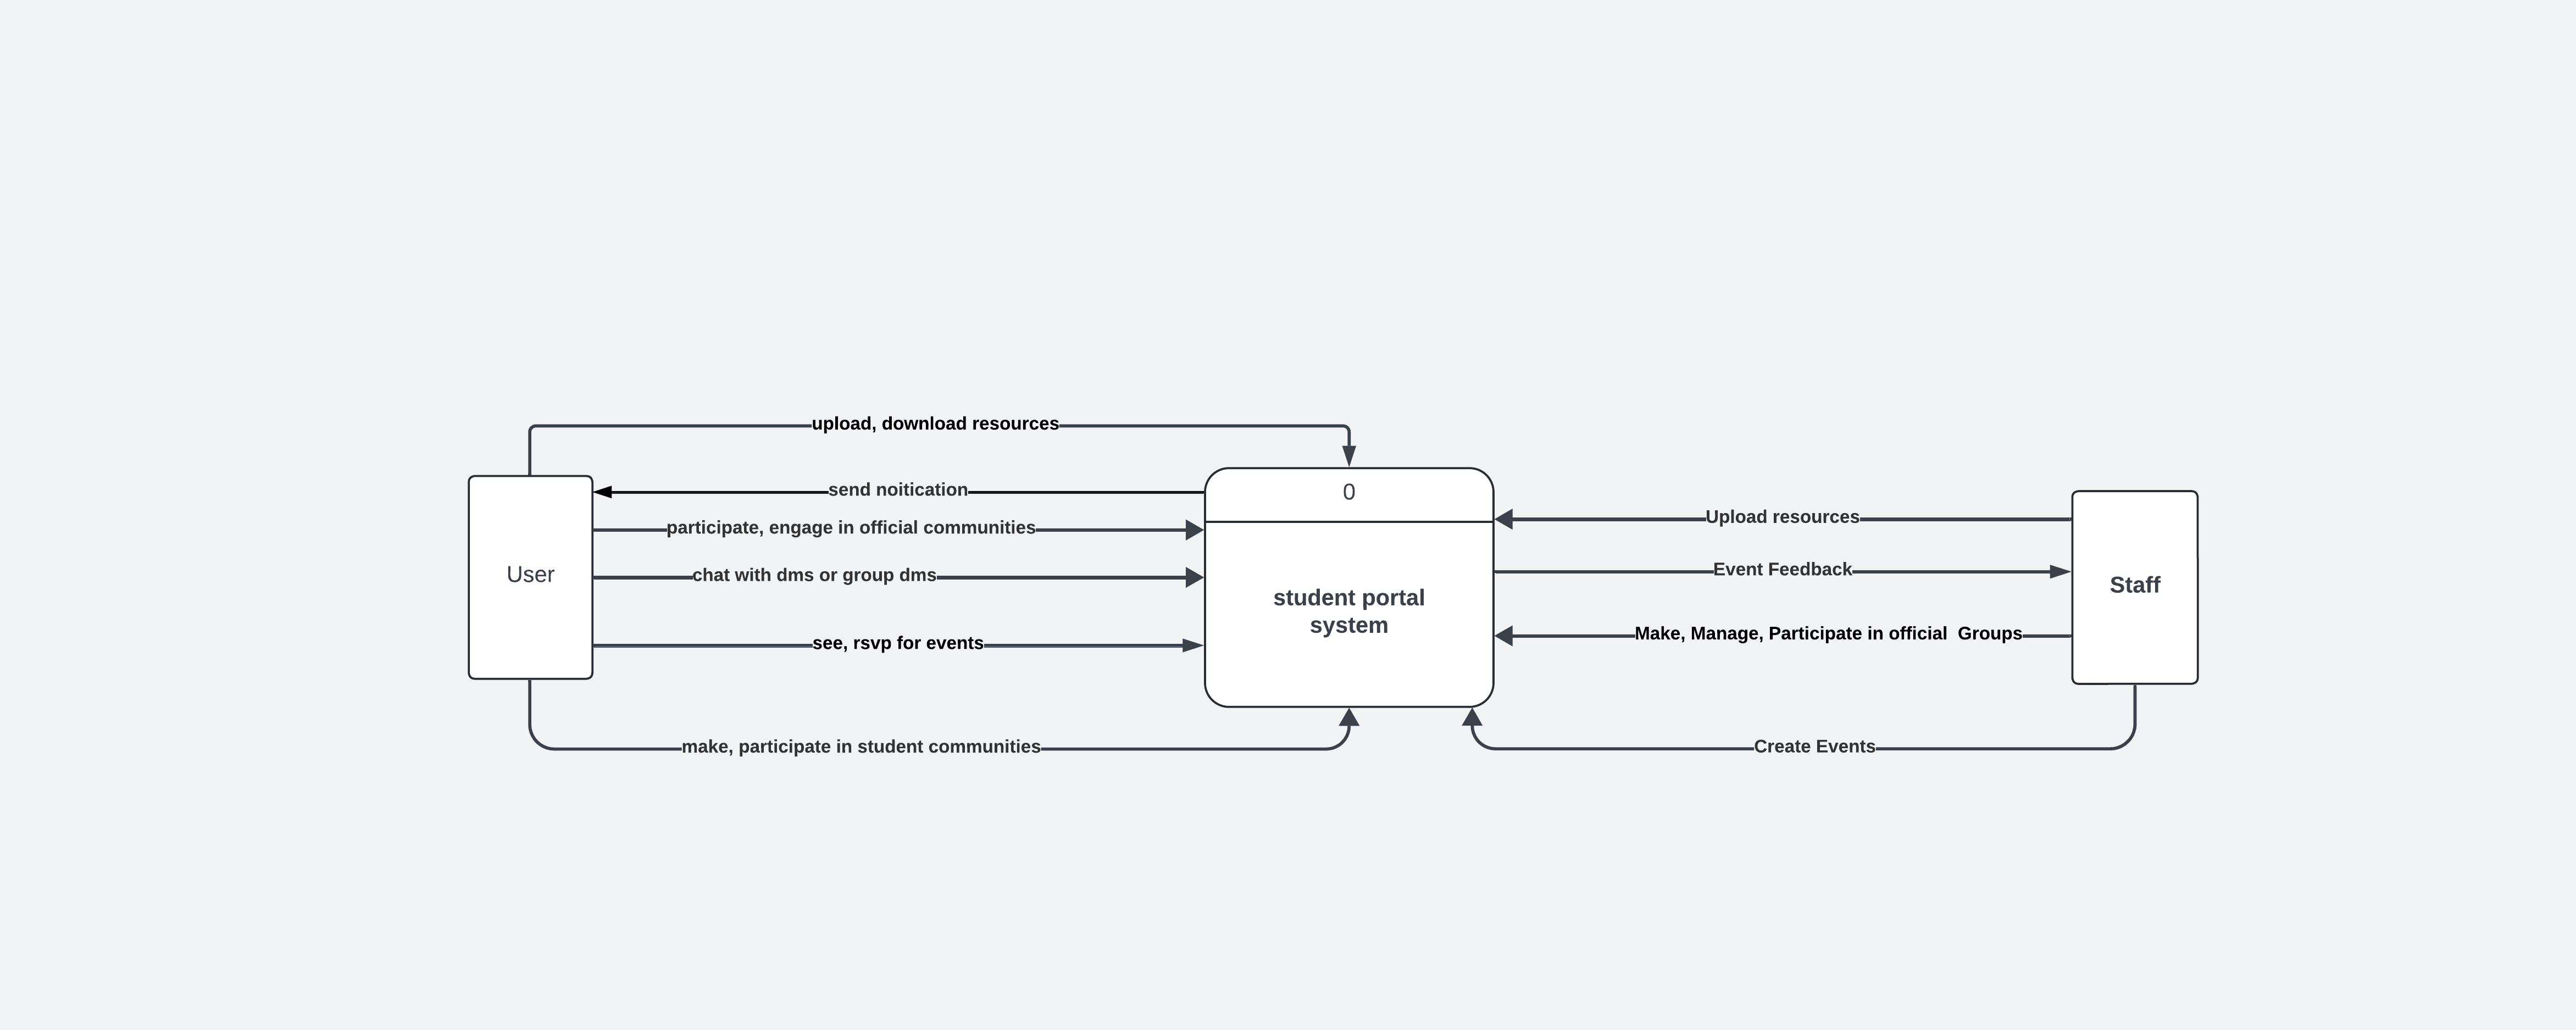
\includegraphics[width=0.8\textwidth]{latex-doc/images/dfd_level0.png}
    \caption{Context diagram showing system boundaries}
    \label{fig:dfd0}
\end{figure}

\subsection{Level 1 DFD}
\begin{figure}[H]
    \centering
    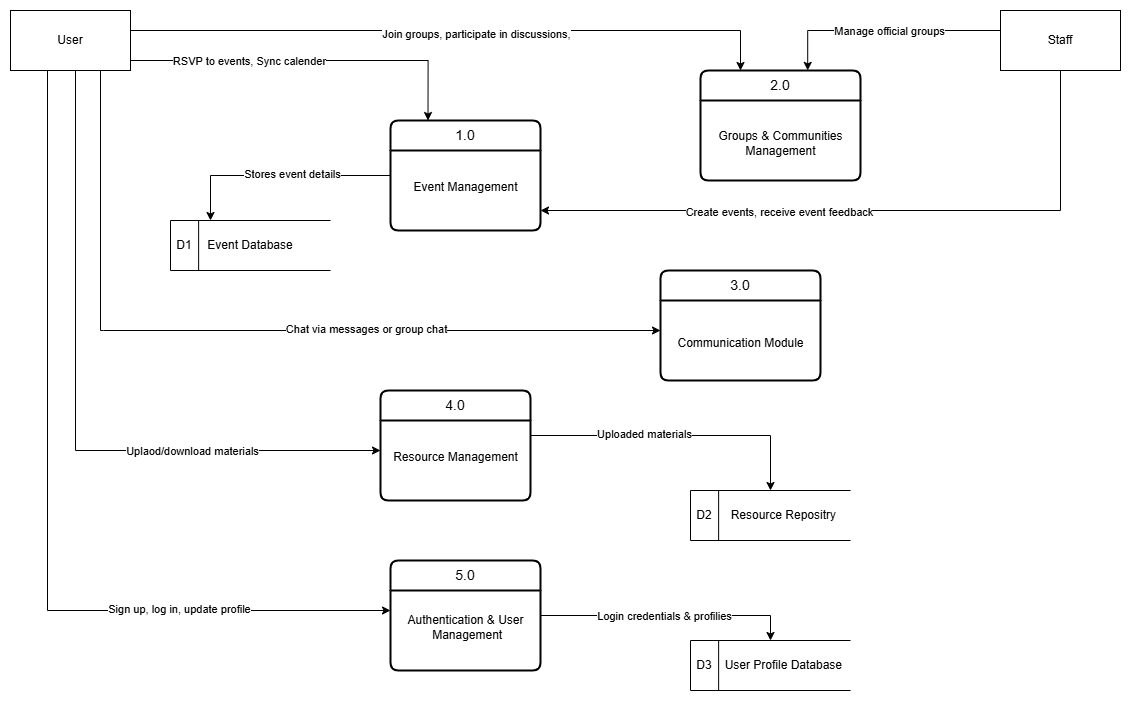
\includegraphics[width=\textwidth]{latex-doc/images/dfd_level1.png}
    \caption{Level 1 DFD showing major subsystems}
    \label{fig:dfd1}
\end{figure}


\vspace{3cm}


\section{Algorithms and Pseudocode}
\label{sec:algorithms}

Key system algorithms are implemented as follows:

\subsection{User Authentication}
\begin{algorithmic}[1]
\State \textbf{Input:} username, password
\State \textbf{Output:} Authentication status (success/failure)
\State
\State Prompt user to enter username and password
\State Retrieve stored hashed password from database for the given username
\If{username exists}
    \State Hash the input password using the same hashing algorithm
    \If{hashed input password matches stored hash}
        \State Grant access to the system
        \State \Return "Authentication successful"
    \Else
        \State \Return "Authentication failed: Incorrect password"
    \EndIf
\Else
    \State \Return "Authentication failed: User not found"
\EndIf
\end{algorithmic}

\subsection{Profile Management}
\begin{algorithmic}[1]
\State \textbf{Input:} userID, updatedProfileData
\State \textbf{Output:} Updated profile status
\State
\State Retrieve user profile using userID
\If{profile exists}
    \State Update profile fields with updatedProfileData
    \State Save changes to the database
    \State \Return "Profile updated successfully"
\Else
    \State \Return "Profile update failed: User not found"
\EndIf
\end{algorithmic}

\subsection{Event Management}
\begin{algorithmic}[1]
\State \textbf{Input:} userID
\State \textbf{Output:} List of events
\State
\State Retrieve events from the database
\State Filter events based on user preferences (if any)
\State Display events to the user
\end{algorithmic}

\vspace{2cm}

\subsection{RSVP for Events}
\begin{algorithmic}[1]
\State \textbf{Input:} userID, eventID
\State \textbf{Output:} RSVP status
\State
\State Check if the event exists in the database
\If{event exists}
    \State Add userID to the event's RSVP list
    \State Update the event in the database
    \State \Return "RSVP successful"
\Else
    \State \Return "RSVP failed: Event not found"
\EndIf
\end{algorithmic}

\subsection{AI-Suggested Events}
\begin{algorithmic}[1]
\State \textbf{Input:} userID
\State \textbf{Output:} List of suggested events
\State
\State Retrieve user preferences and past event attendance
\State Use AI model to predict events of interest
\State \Return list of suggested events
\end{algorithmic}

\subsection{Resource Sharing}
\begin{algorithmic}[1]
\State \textbf{Input:} userID, resourceFile, category
\State \textbf{Output:} Upload status
\State
\State Upload resourceFile to the server
\State Store resource metadata in the database
\State \Return "Resource uploaded successfully"
\end{algorithmic}

\subsection{Discussion Participation}
\begin{algorithmic}[1]
\State \textbf{Input:} userID, discussionID, message
\State \textbf{Output:} Participation status
\State
\State Retrieve discussion using discussionID
\If{discussion exists}
    \State Add message to the discussion
    \State Update discussion in the database
    \State \Return "Message posted successfully"
\Else
    \State \Return "Discussion not found"
\EndIf
\end{algorithmic}

\vspace{2cm}

\subsection{AI-Powered Chatbot}
\begin{algorithmic}[1]
\State \textbf{Input:} userQuery
\State \textbf{Output:} Chatbot response
\State
\State Analyze userQuery using NLP
\State Retrieve most relevant response from FAQ database
\State \Return response to the user
\end{algorithmic}

\subsection{Recommendation Engine}
\begin{algorithmic}[1]
\State \textbf{Input:} userID
\State \textbf{Output:} List of recommended content
\State
\State Retrieve user preferences and past interactions
\State Use collaborative filtering algorithm
\State \Return list of recommended content
\end{algorithmic}

\subsection{Announcements Dashboard}
\begin{algorithmic}[1]
\State \textbf{Description:} Displays important announcements and updates to users
\State
\State \textbf{Input:} userID
\State \textbf{Output:} List of announcements
\State
\State Retrieve announcements from the database
\State Filter announcements based on user preferences (if any)
\State Display announcements to the user
\end{algorithmic}

\subsection{Direct Messaging}
\begin{algorithmic}[1]
\State \textbf{Description:} Allows users to send direct messages to mentors or peers
\State
\State \textbf{Input:} senderID, receiverID, message
\State \textbf{Output:} Message send status (success/failure)
\State
\State Store message in the database with senderID, receiverID, and timestamp
\State Notify receiver of the new message
\State \Return "Message sent successfully"
\end{algorithmic}

\subsection{Categorized Content Upload}
\begin{algorithmic}[1]
\State \textbf{Description:} Allows users to upload content under specific categories
\State
\State \textbf{Input:} userID, contentFile, category
\State \textbf{Output:} Content upload status (success/failure)
\State
\State Upload contentFile to the server
\State Store content metadata (userID, category, timestamp) in the database
\State \Return "Content uploaded successfully"
\end{algorithmic}

\subsection{Sync with Personal Calendars}
\begin{algorithmic}[1]
\State \textbf{Description:} Allows users to sync event dates with personal calendars
\State
\State \textbf{Input:} userID, eventID
\State \textbf{Output:} Sync status (success/failure)
\State
\State Retrieve event details using eventID
\If{event exists}
    \State Add event to user's personal calendar (Google Calendar, Outlook)
    \State \Return "Sync successful"
\Else
    \State \Return "Sync failed: Event not found"
\EndIf
\end{algorithmic}

\subsection{View Events}
\begin{algorithmic}[1]
\State \textbf{Description:} Allows users to view academic events
\State
\State \textbf{Input:} userID
\State \textbf{Output:} List of events
\State
\State Retrieve events from the database
\State Filter events based on user preferences (if any)
\State Display events to the user
\end{algorithmic}

\subsection{Mentorship Matching}
\begin{algorithmic}[1]
\State \textbf{Input:} userID
\State \textbf{Output:} Matched mentor
\State
\State Retrieve user profile and preferences
\State Calculate compatibility scores with potential mentors
\State \Return best matching mentor
\end{algorithmic}

\subsection{Real-Time Notifications}
\begin{algorithmic}[1]
\State \textbf{Input:} userID, notificationMessage
\State \textbf{Output:} Notification status
\State
\State Send notificationMessage to user's device
\State Store notification in the database
\State \Return "Notification sent successfully"
\end{algorithmic}

\section{Interface Design}
\label{sec:interface_design}

\subsection{Mobile Application Interfaces}
\begin{figure}[H]
    \centering
    % First row
    \begin{subfigure}{0.3\textwidth}
        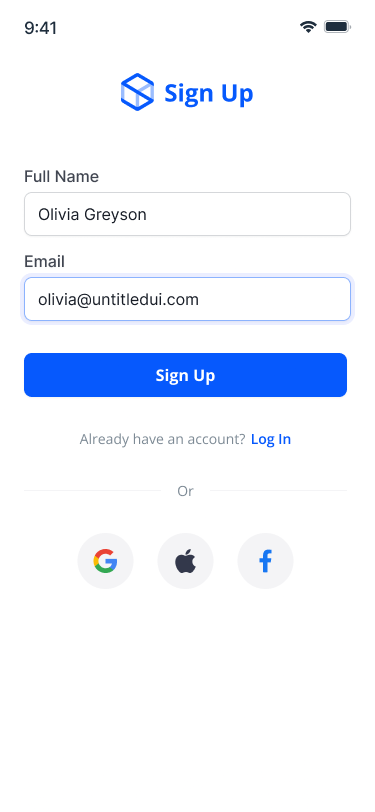
\includegraphics[width=\linewidth]{latex-doc/images/mobile_interface/Sign-up.png}
        \caption{Registration flow}
        \label{fig:signup}
    \end{subfigure}
    \hfill
    \begin{subfigure}{0.3\textwidth}
        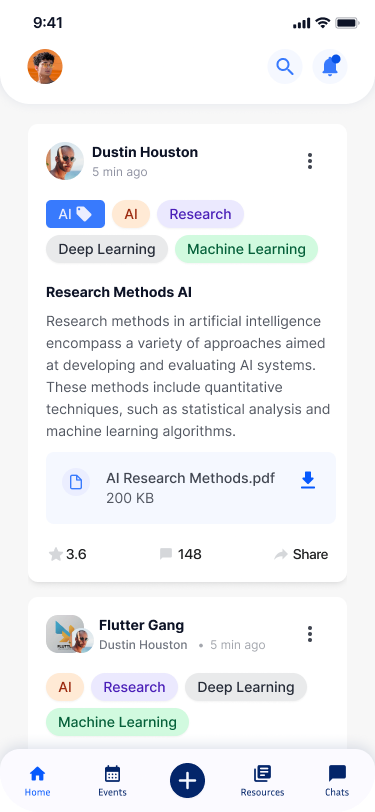
\includegraphics[width=\linewidth]{latex-doc/images/mobile_interface/Home.png}
        \caption{Main activity feed}
        \label{fig:home}
    \end{subfigure}
    \hfill
    \begin{subfigure}{0.3\textwidth}
        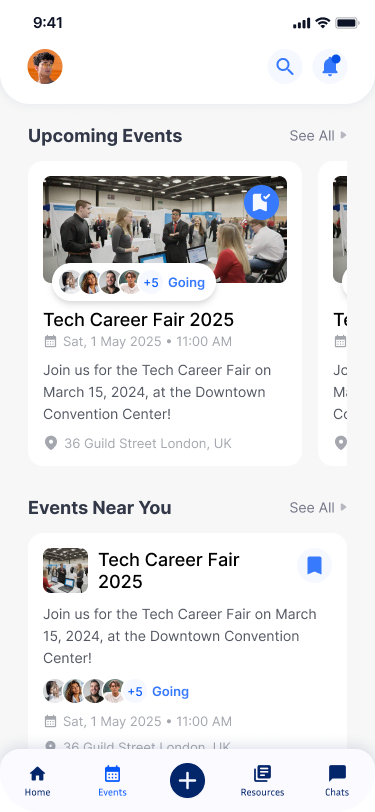
\includegraphics[width=\linewidth]{latex-doc/images/mobile_interface/Events.png}
        \caption{Event discovery}
        \label{fig:events}
    \end{subfigure}
    \vspace{0em} % spacing between rows

    % Second row
    \hfill
    \begin{subfigure}{0.3\textwidth}
        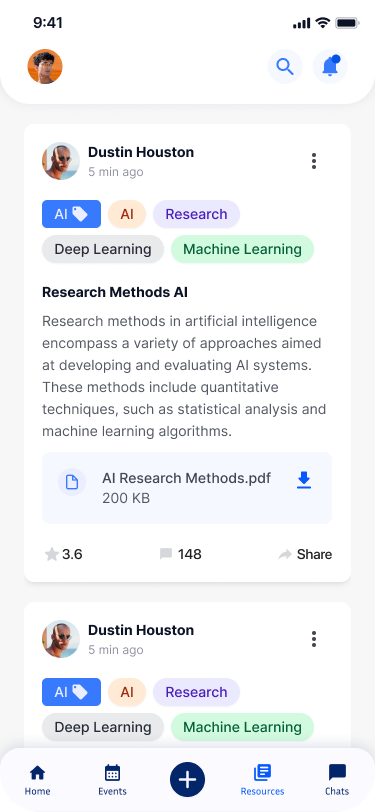
\includegraphics[width=\linewidth]{latex-doc/images/mobile_interface/Resources.png}
        \caption{Academic resources}
        \label{fig:resources}
    \end{subfigure}
    \hfill
    \begin{subfigure}{0.3\textwidth}
        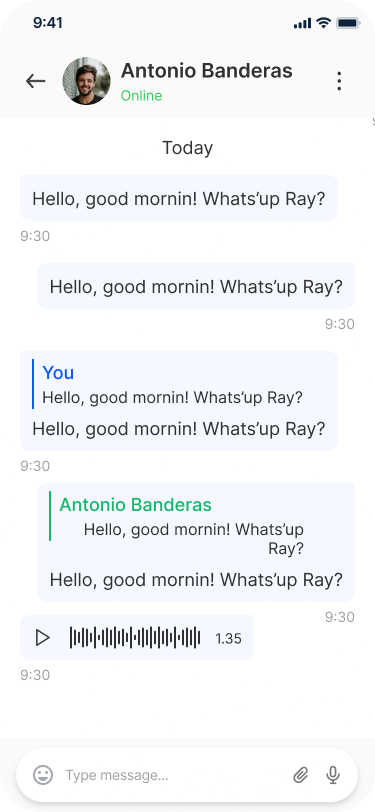
\includegraphics[width=\linewidth]{latex-doc/images/mobile_interface/Chat.png}
        \caption{Messaging interface}
        \label{fig:chat}
    \end{subfigure}
    \hfill
    \begin{subfigure}{0.3\textwidth}
        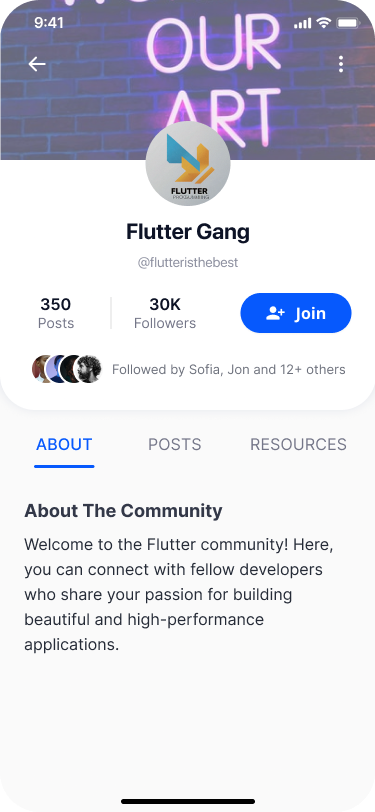
\includegraphics[width=\linewidth]{latex-doc/images/mobile_interface/General-Profile.png}
        \caption{User profile}
        \label{fig:profile}
    \end{subfigure}

    \caption{Mobile Application Interfaces Overview}
    \label{fig:mobile_interfaces}
\end{figure}


\subsection{Admin Dashboard Interfaces}
\begin{figure}[H]
    \centering
    \begin{subfigure}{0.45\textwidth}
        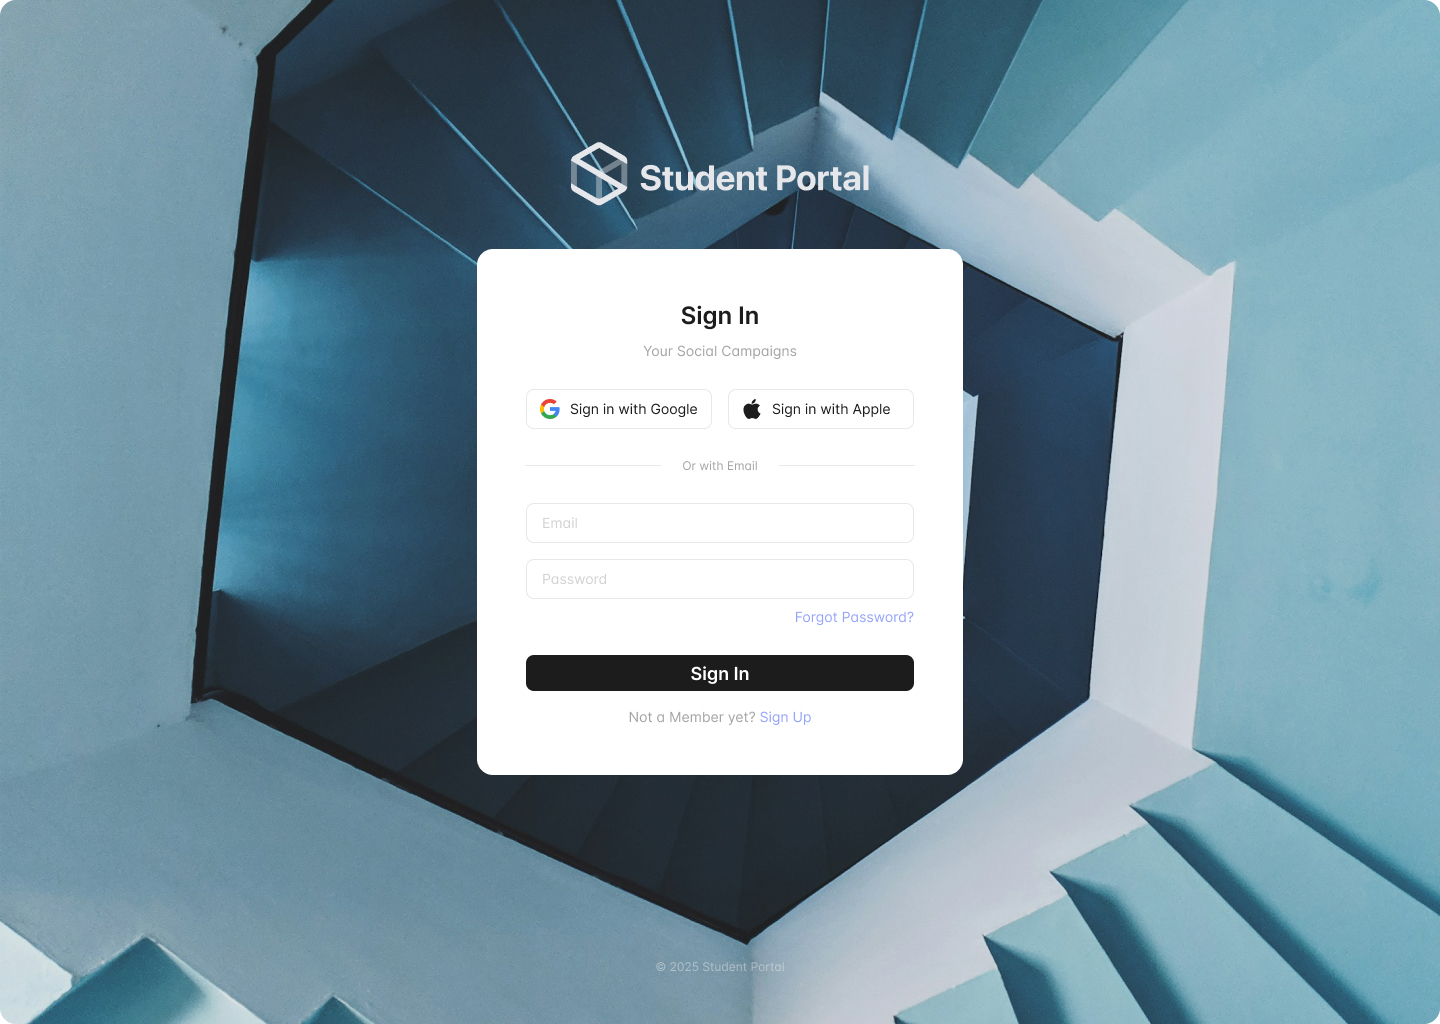
\includegraphics[width=\textwidth]{latex-doc/images/web_interface/Authentication-Sign_In.jpg}
        \caption{Admin login screen}
        \label{fig:admin_login}
    \end{subfigure}
    \begin{subfigure}{0.45\textwidth}
        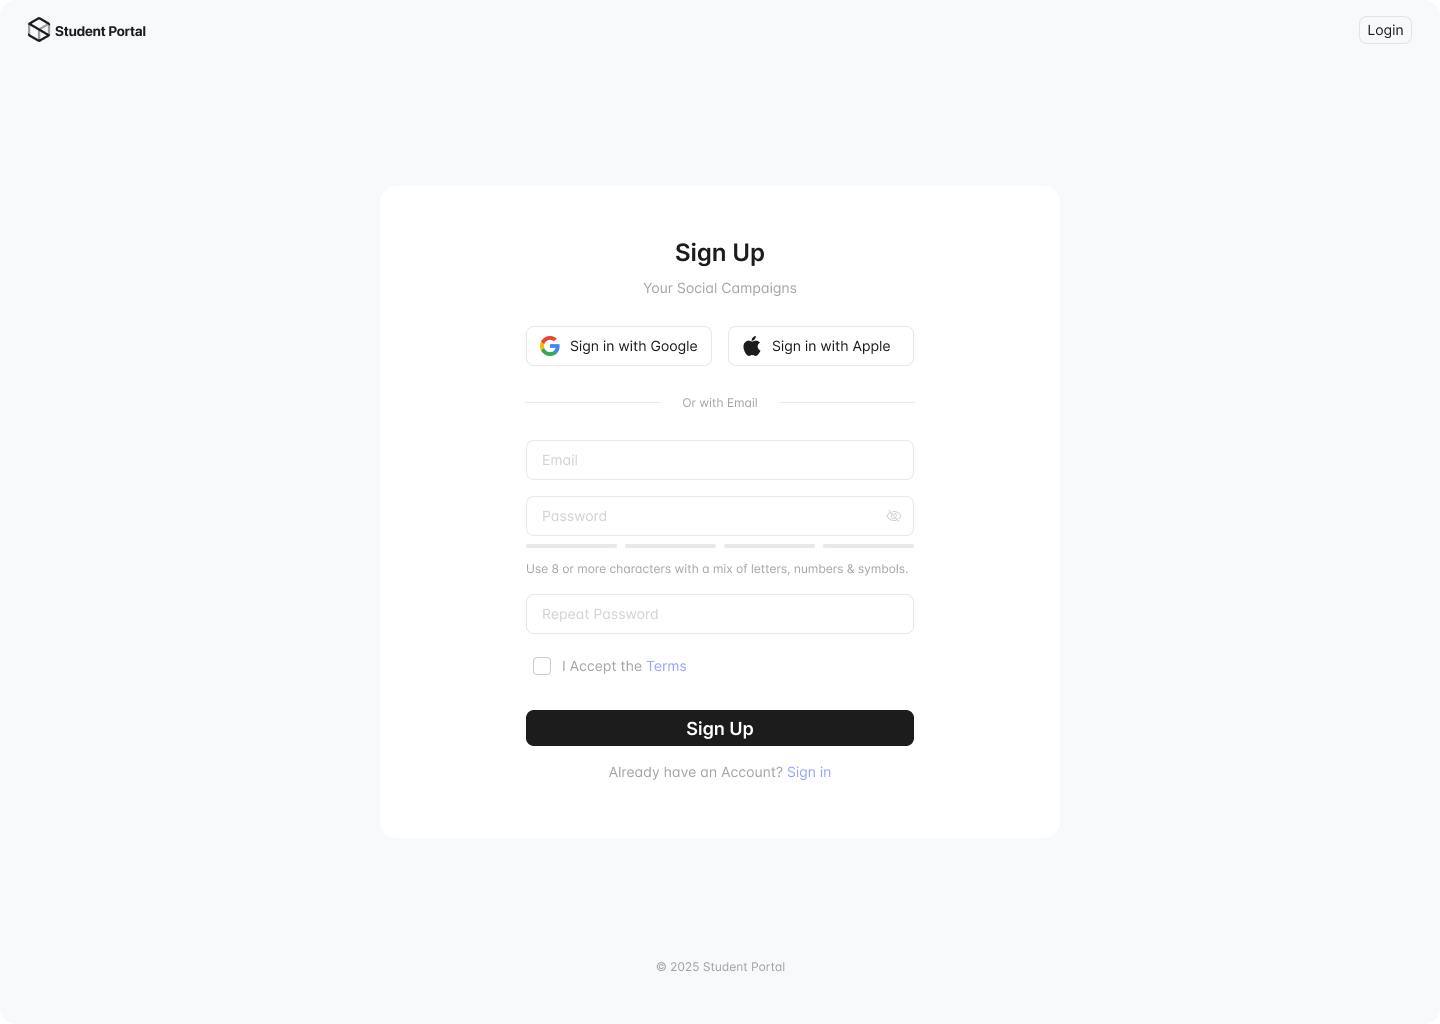
\includegraphics[width=\textwidth]{latex-doc/images/web_interface/Authentication-Sign_Up.jpg}
        \caption{Admin account creation}
        \label{fig:admin_signup}
    \end{subfigure}
    \caption{Admin portal authentication flows}
    \label{fig:admin_auth}
\end{figure}

\begin{figure}[H]
    \centering
    \begin{subfigure}{0.45\textwidth}
        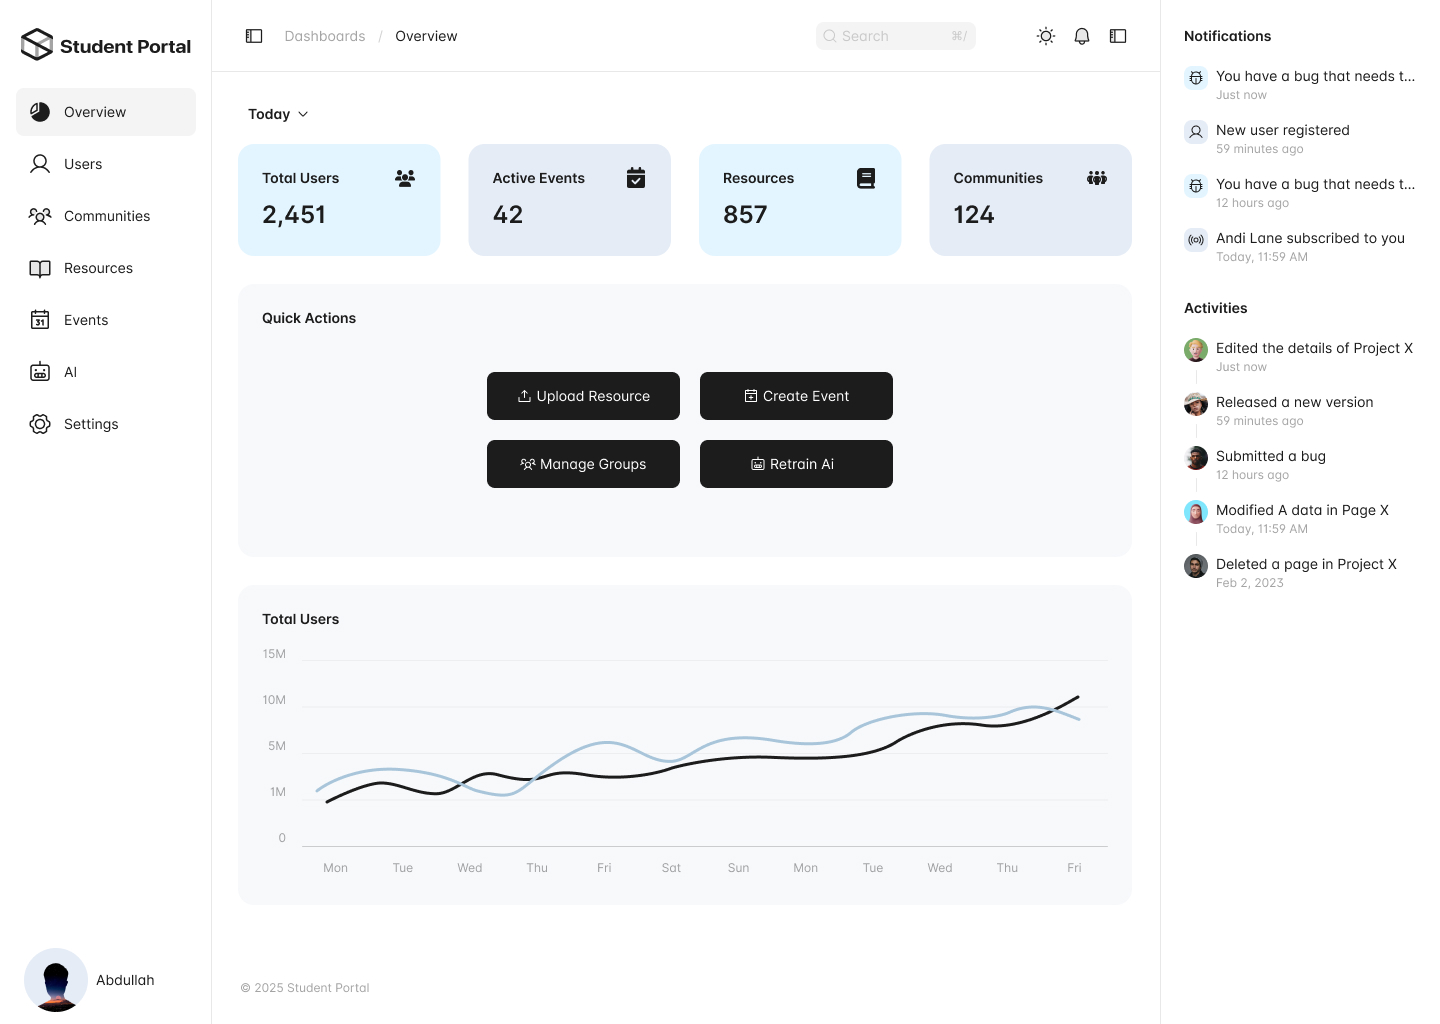
\includegraphics[width=\textwidth]{latex-doc/images/web_interface/Overview.jpg}
        \caption{Dashboard overview}
        \label{fig:overview}
    \end{subfigure}
    \begin{subfigure}{0.45\textwidth}
        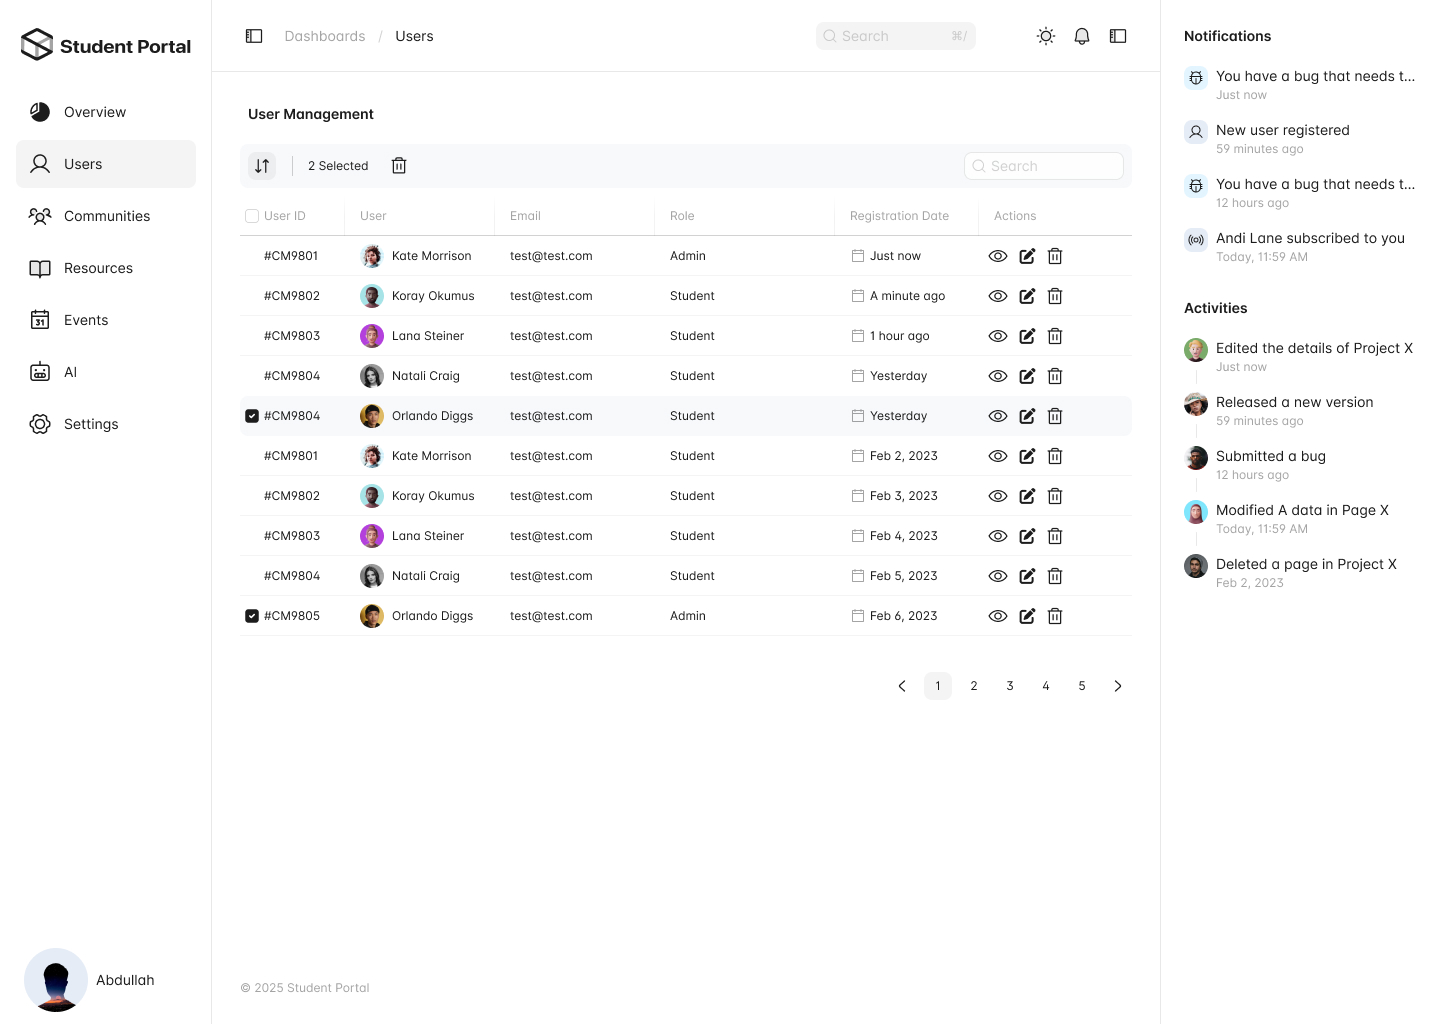
\includegraphics[width=\textwidth]{latex-doc/images/web_interface/User-Management.jpg}
        \caption{User management console}
        \label{fig:user_mgmt}
    \end{subfigure}
    \caption{Admin dashboard main views}
    \label{fig:admin_main}
\end{figure}

\begin{figure}[H]
    \centering
    \begin{subfigure}{0.45\textwidth}
        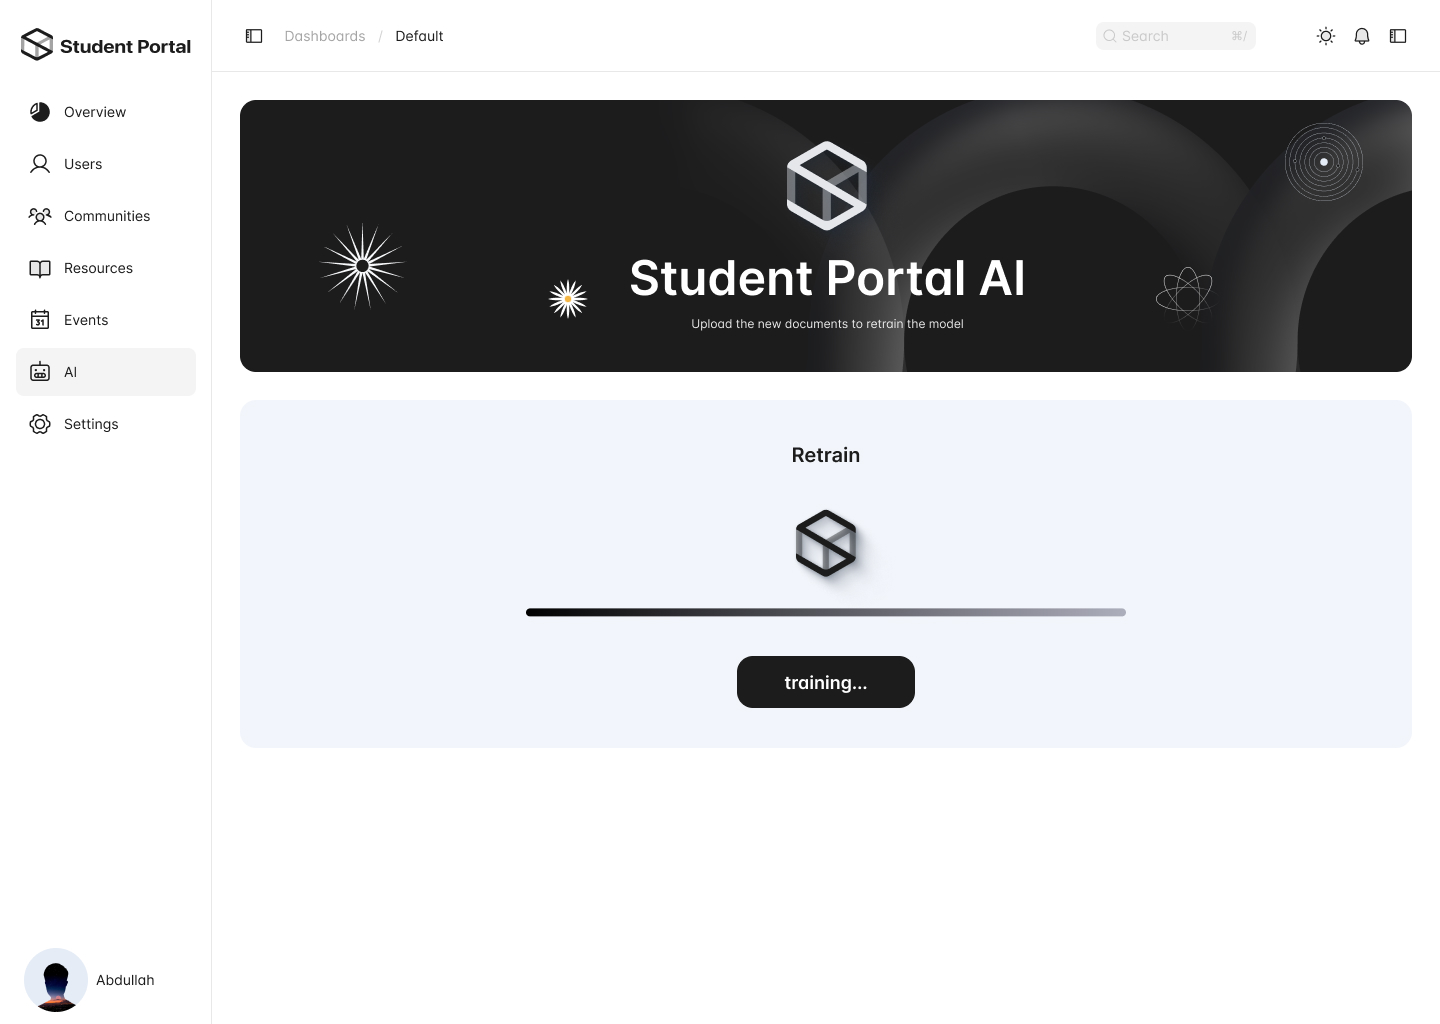
\includegraphics[width=\textwidth]{latex-doc/images/web_interface/AI-training.jpg}
        \caption{AI model training interface}
        \label{fig:ai_training}
    \end{subfigure}
    \begin{subfigure}{0.45\textwidth}
        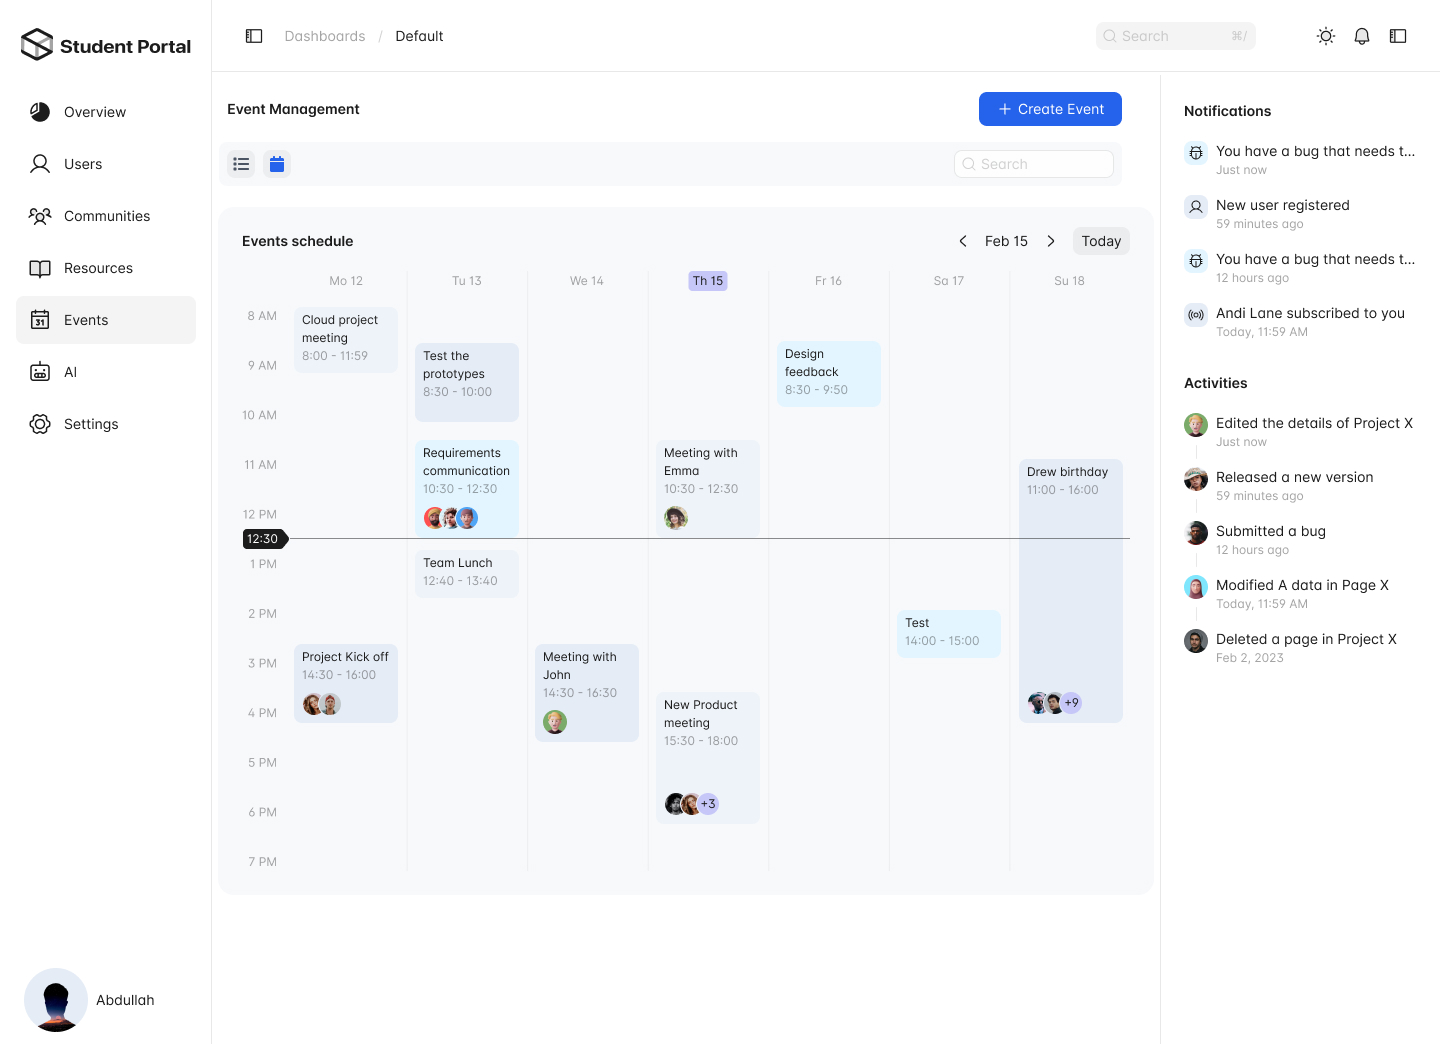
\includegraphics[width=\textwidth]{latex-doc/images/web_interface/Event-Management-cal.jpg}
        \caption{Event moderation panel}
        \label{fig:event_mgmt}
    \end{subfigure}
    \caption{Specialized admin tools}
    \label{fig:admin_tools}
\end{figure}
